\documentclass[a4paper]{article}

\renewcommand{\rmdefault}{ftm} % Times New Roman
\usepackage[12pt]{extsizes} % для того чтобы задать нестандартный 12-ый размер шрифта

\renewcommand{\scriptsize}{\fontsize{14}{14pt}\selectfont}
\usepackage{titlesec}
\titleformat{\section}
    {\normalsize\scriptsize\bfseries}
    {\thesection}
    {1em}{\scriptsize\bfseries}   
\titleformat{\subsection}
    {\normalsize\scriptsize\bfseries}
    {\thesubsection}
    {1em}{\scriptsize\bfseries}
\titleformat{\subsubsection}
    {\normalsize\scriptsize\bfseries}
    {\thesubsubsection}
    {1em}{\scriptsize\bfseries}

\usepackage{extsizes}
\usepackage{physics}
\usepackage{latexsym} 
\usepackage[left=30mm, top=20mm, right=15mm, bottom=20mm]{geometry}
\usepackage{indentfirst}
\setlength{\parindent}{1.25cm}
\usepackage{lscape}
\usepackage{float}
%%% Дополнительная работа с математикой
\usepackage{amsmath,amsfonts,amssymb,amsthm,mathtools} % AMS
\usepackage{icomma} % "Умная" запятая: $0,2$ --- число, $0, 2$ 

%%%% Работа с русским языком
\usepackage{cmap}					% поиск в PDF
\usepackage{mathtext} 				% русские буквы в формулах
\usepackage[T2A]{fontenc}			% кодировка
\usepackage[utf8]{inputenc}			% кодировка исходного текста
\usepackage[english,russian]{babel}	% локализация и переносы


%%% Добавлена поддержка для кастомизации таблиц
\usepackage[table,xcdraw]{xcolor}
\usepackage{booktabs}

%%% Работа с картинками
\usepackage{graphicx}  % Для вставки рисунков
\graphicspath{{image/}}  % папки с картинками
\setlength\fboxsep{3pt} % Отступ рамки \fbox{} от рисунка
\setlength\fboxrule{1pt} % Толщина линий рамки \fbox{}
\usepackage{wrapfig} % Обтекание рисунков и таблиц текстом


\usepackage[backend=biber,style=numeric,sorting=none]{biblatex}
\usepackage{csquotes}
%\addbibresource{bibleograf.bib}


\linespread{1.3}
%\pagestyle{plain}

%для замены двоеточия на тире после номера рисунка и таблицы 
\usepackage{ccaption}
% заменяем для рисунков ':' после номера рисунка на '.'
\captiondelim{ -- } % после точки стоит пробел!

% biber
\usepackage[backend=biber,style=numeric,sorting=none]{biblatex}
\usepackage{csquotes}
\addbibresource{books.bib}

%%%%%%%%%%%%%%%%%%%%%%%%%%%%%%%%%%%%%%%%%%%%%%%%%%%%%%%%%%%%%%%%%%%%%%%%%%%%%%%%%%%%%%%%%%%

\begin{document}
\begin{center}
\small
Федеральное государственное автономное образовательное учреждение высшего образования\\
<<Московский физико-технический институт (Национальный исследовательский университет)>> \\
Физтех-школа аэрокосмических технологий\\
Кафедра теоретической и экспериментальной физики геосистем
\end{center}

\begin{flushleft}
\small
\textbf{Направление подготовки:} 03.03.01 Прикладные математика и физика (бакалавриат)\\
\textbf{Направленность(профиль) подготовки:} Физика и механика космических и природных систем\\
\end{flushleft}

\begin{center}
\LARGE
\textbf{Пространственно-временное распределение полного электронного содержания в различных геофизических условиях}

\small(бакалаврская работа)
\end{center}


\begin{flushright}

\noindent
\textbf{Студент:} \\
Скачков Алексей Павлович\\
\underline{\hspace{3cm}}\\
\textbf{Научный руководитель:}\\
Ряховский Илья Александрович\\
\underline{\hspace{3cm}}\\

\end{flushright}

\begin{center}
\small
Москва\\
2020
\end{center}

%%%%%%%%%%%%%%%%%%%%%%%%%%%%%%%%%%%%%%%%%%%

\newpage
\section*{Аннотация}

\subsection*{Цели и задачи}
Целью данной работы является получение пространственно-временного распределения полного электронного содержания во время солнечной вспышки 10 сентября 2017 года.\\


Для достижения поставленной цели решались следующие задачи:
\begin{itemize}
\item Обработка данных со станций GNSS
\item Вычисление наклонного ПЭС по групповым и фазовым измерениям
\item Оценка вертикального значения ПЭС
\item Нахождение пространственных и временных зависимостей изменения ПЭС
\end{itemize}

\subsection*{Полученные результаты}
Результатами являются подтверждение работоспособности метода вычисление значения полного электронного содержания, представленного в данной работе, верификация данных, полученных этим методом, и получение пространственно-временных зависимостей изменения абсолютного значения полного электронного содержания вследствие воздействия солнечной вспышки, подтверждающих влияние вспышек на состояние ионосферы.

\newpage
\tableofcontents

\newpage
\section*{Используемые обозначения}

\newpage
\section*{Введение}
\addcontentsline{toc}{section}{Введение}
\subsection*{Актуальность темы}
Исследование ионосферы является достаточно важным направлением, так как от ее состояния зависит множество факторов, влияющих на нашу повседневную жизнь. Знание о состоянии ионосферы может помогать идентифицировать различные события техногенного и естественного характеров. В современной действительности стало ясно, что различные ионосферные процессы влияют на погодные и климатические условия. Не стоит забывать и о современных средствах связи, навигации и локации, которые напрямую зависят от состояния ионосферы.

\subsection*{Объект исследования}
Основные параметры, характеризующие ионосферу: локальная электронная концентрация $N_e$, температура ионов и электронов и полное электронное содержание.

Объектом исследования данной работы является полное электронное содержание (ПЭС или TEC в англоязычной литературе). ПЭС представляет собой количество электронов в столбе единичного сечения. В рамках данной работы предлагается получение пространственно-временного распределения полного электронного содержания во время высокой солнечной активности.

\subsection*{Значимость исследования}


\newpage
\section{Теоретические сведения}
\subsection{Использование GPS в исследовании ионосферы}
Существует множество различных методов, применяемых для исследования состояния ионосферы, такие как вертикальное, наклонное, вертикально-наклонное, внешнее зондирования, некогерентное рассеяние и многие другие. Появление глобальной навигационной системы и создание огромной сети GPS станций стали началом новой эры дистанционного исследования ионосферы. Большое количество станций и непрерывная доступность спутников позволяют производить своевременный мониторинг ионосферы в различных участках планеты. 

\subsection{Общие сведения о GPS}
GPS (Global Positioning System) представляет из себя спутниковую систему навигации, которая обеспечивает измерение расстояния между спутником и приемником, а так же времени. На основе этих данных определяется местоположение объекта в пространстве.

Систему GPS можно разделить на три основные составляющие:
\begin{itemize}
\item Космический сегмент
\item Сегмент управления
\item Сегмент потребителей
\end{itemize}

\textbf{Космический сегмент} состоит из $32$ спутников (один из которых находится на этапе развертки)\footnote{на момент Февраля 2019 года \cite{gpsgov}}, которые размещены на шести круговых орбитах. Высота орбит составляет $20200$ км. Наклонение орбит также являет общим и равно $55^{\circ}$. Каждая орбита разнесена друг относительно друга на $60^{\circ}$ по долготе. Спутники оборудованы специальным устройством, которое хранит системное время аппарата. Временные шкалы всех спутников согласованы между собой и синхронизируются системой единого времени.

Спутники непрерывно передают сигналы на двух частотах: $f_1 = 1575.42 \text{ МГц}$ и $f_2 = 1227.60 \text{ МГц}$. Передаваемые сигналы модулируются псевдослучайными последовательностями (PRN - Pseudorandom Noise) двух типов C/A-код и P-код.

C/A-код является открытым кодом, который, в основном, используется в гражданских целях. Он имеет длину повторения 1 мс и частоту следования импульсов $1.023 \text{ МГц}$.

P-код - это защищенный код. Частота следования имеет значение $10.23 \text{ МГц}$ и длину в 267 суток. Сигналы, модулированные P-кодом, передаются на двух частотах $f_1$ и $f_2$, в то время как C/A-код только на $f_1$.

Вместе с PRN-кодами также отправляются навигационные сообщения, которые содержат данные о положении спутника, метки времени, частотно-временные поправки, сведения о работоспособности оборудования и др.

\textbf{Сегмент управления} осуществляет слежение за орбитальными аппаратами и управление ими. Главная станция находится в Колорадо-Спрингс, штат Колорадо. Станции слежения выполняют измерения траекторий по сигналам спутников и после корректируют поведение каждого спутника.

\textbf{Сегмент потребителей} состоит из устройств разной степени сложности, от военного оборудования до гражданских мобильных устройств. GPS-приемники производят выбор рабочего созвездия (набора из не менее 4 видимых спутников), поиск, слежение и декодировку входящего сигнала, обработку измеряемых радионавигационных параметров и служебной информации, расчет координат и скорости потребителя.

\subsection{Интересующие виды измерений в GPS}
Основная величина, которая измеряется в спутниковых системах позиционирования, является <<псевдодальность>>, через которую определяют координаты GPS-приемника.

\begin{equation}
D' = \sqrt{(x - x_S)^2 + (y - y_S)^2 + (z - z_S)^2} + c\tau_R +\sigma_D,
\end{equation}
где $D'$ - <<псевдодальнось>> между приемником и спутником; $x_S, y_S, z_S$ -- координаты спутника; $x, y, z$ -- координаты приемника; $c$ -- скорость света; $\tau_R$ - отклонение часов приемника от системного времени GPS; $\sigma_D$ -- погрешность измерения. 
Псевдодальность отличается от действительного расстояния $D = \sqrt{(x - x_S) ^ 2 + (y - y_S) ^ 2 + (z - z_S) ^ 2}$ наличием ошибок измерений. 
Зная значения псевдодальности для 4 спутников, можно вычислить координаты приемника и значение $\tau_R$. Нахождение данных величин возможно в любой момент времени, так как в поле зрения приемника всегда оказывается минимум 5 спутников. В современных устройствах для вычисления положения в пространстве используется метод взвешенных наименьших квадратов. Для определения псевдодальности измеряются такие параметры, как время распространения сигнала и набег фазы несущей радиоволны на трассе <<спутник -- приемник>>. В зависимости от выбранного параметра различают кодовые и фазовые измерения псевдодальности.

\textbf{Кодовые измерения псевдодальности.} $D' = c \tau$. В данном случае измеряется время задержки между моментом излучения и момента получения сигнала, т.е. время распространения сигнала. Для измерения задержки, с помощью корреляционного анализа, определяется сдвиг выбранного кода, посланного спутником, относительно кода, генерируемого приемным устройством. Таким образом, двухчастотный приемник имеет возможность измерять псевдодальность тремя способами: с помощью C/A-кода на частоте $f_1$ и по P-коду на частотах $f_1$ и $f_2$\footnote{измерение по C/A-коду обозначается как $C1$, а для P-кода соответственно $P1$ и $P2$}. Точность определения псевдодальности по кодовым измерениям составляет $1\%$ от длины кода, что позволяет делать измерение по C/A-коду с погрешностью в 3 метра, а по P-коду c погрешностью 0.3 метра.

\textbf{Фазовые измерения псевдодальности.} $D' = \lambda \Delta \varphi + \lambda \text{N}$. Для получения пседодальности в этом случае измеряется разность фаз $\Delta\varphi$ двух несущих радиоволн: принятой приемником и сгенерированной в самом приемнике; $\lambda = c / f$ -- длина волны несущей частоты. Для фазовых измерений на частотах $f_1$ и $f_2$ приняты обозначения $L1$ и $L2$ соответственно. Полное число циклов фазы N остается неизвестной величиной. Этому дали название <<фазовой неоднозначностью измерений>>. Для ее устранения существует ряд способов, одним из которых является комбинирование кодовых и фазовых измерений. Погрешность измеренной разности фаз $\Delta\varphi$ имеет точность до 0.01 периода. Тогда псевдодальность может быть определена с точностью до 1-2 мм.

\textbf{Погрешности измерений.} На точность измерений влияет множество факторов, которые представлены в таблице \ref{tableErrors} \cite{hoffmanErrors}, \cite{shebshaevich}.

% Таблица с данными о погрешности
\begin{table}[h]
\begin{center}
\begin{tabular}{|l|l|}
\hline
\rowcolor[HTML]{DAE8FC} 
{\color[HTML]{000000} \textbf{Источник погрешности}}                                                                                     & {\color[HTML]{000000} \textbf{Вносимая погрешность}} \\ \hline
Геометрическое расположение НИСЗ                                                                                                         & PDOP                                                 \\ \hline
Неточности расчетов орбит НИСЗ и времени                                                                                                 & 0.5 -- 3 м                                           \\ \hline
Случайные отклонения опбит и часов                                                                                                       & 0.5 -- 3 м                                           \\ \hline
Шумы приемника                                                                                                                           & 1.5 -- 3 м                                           \\ \hline
Задержка сигнала в ионосфере                                                                                                             & 2 -- 10 м                                            \\ \hline
Задержка сигнала в тропосфере                                                                                                            & 1 -- 2 м                                             \\ \hline
\begin{tabular}[c]{@{}l@{}}Многолучевость распространения\\ (в результате отражений от крупных объектов\\ вблизи приемника)\end{tabular} & 1 -- 2 м                                             \\ \hline
\begin{tabular}[c]{@{}l@{}}Меры по искусственному снижению точности \\ (с Мая 2000 года не используется)\end{tabular}                    & до 30 м                                              \\ \hline
Прочие источники                                                                                                                         & 1 м                                                  \\ \hline
\end{tabular}
\end{center}
\caption{Составляющие погрешности навигационных определений}
\label{tableErrors}
\end{table}

Наиболее важным фактором для получения хорошей точности является геометрия рабочего созвездия спутников. Для характеристики взаимного расположения приемника и спутника вводится коэффициент PDOP (Position Dilution of Precision)\footnote{Величина PDOP обратно пропорциональна объему фигуры, образованной пересечение лучей <<спутник -- приемник>> со сферой единичного радиуса, центр которой совмещен с приемником.}. На данный коэффициент умножается все другие ошибки. 

Вторым по значимости фактором, снижающим точность, является ионосферная задержка радиосигнала. Именно из-за этого эффекта GPS может использоваться для исследования состояния ионосферы.

Для снижения ионосферной и тропосферной погрешностей измерений используются математические модели, комбинирование данных, сглаживание данных и режим DGPS\footnote{суть метода заключается в том, что измерения производятся двумя приемниками, один из которых неподвижен (для него известно истинное положение). Неподвижный приемник сравнивает свое истинное положение с положением, полученным с GPS, и отправляет поправочные коэффициенты второму приемнику.}.

Комбинация кодовых и фазовых измерений и использование их в алгоритмах сглаживания данных позволяют эффективно фильтровать погрешности, связанные с геометрией рабочего созвездия, шумами приемника, случайными отклонениями орбит часов и многолучевостью. 

\subsection{Геометрические положения, используемые для GPS зондирования}
Для расчета полного электронного содержания необходимо знать направление на спутник. На рисунке \ref{pic1}, можно увидеть схематическое представление геометрии системы <<Земля -- спутник>>.

\begin{figure}[!h]
\centering
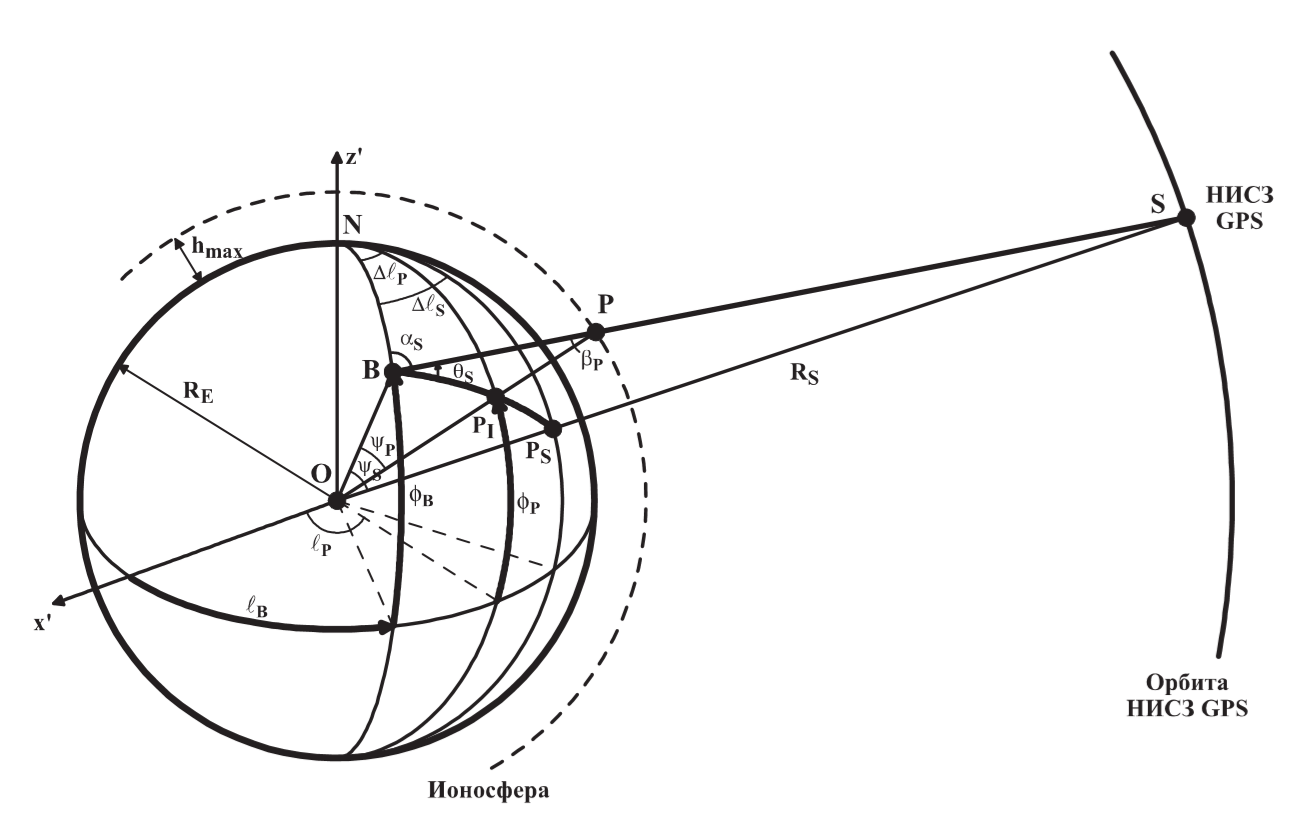
\includegraphics[width = \linewidth]{pics/pic1.png}
\caption{Геометрия системы <<Земля -- спутник>>: $O$ -- центр Земли; $S$ -- спутник; $B$ -- пункт наблюдения; $P$ -- ионосферная точка; $P_I$ -- подионосферная точка; $P_S$ -- подспутниковая точка; $h_\text{max}$ -- высота максимума слоя F2 ионосферы. \cite{afraimovich}}
\label{pic1}
\end{figure}

Для вычисления координат $\alpha_S$, $\theta_S$, которые являются, соответственно, азимутом и углом места (элевация), используется метод расчета на основе геодезических координат спутника и точки наблюдения. С достаточной для практических целей точностью азимут и угол места могут быть вычислены с помощью формул \cite{kotyashkin}:

\begin{equation}
	\begin{aligned}
	&\alpha_S = \arccos{\left(\frac{\sin{\Phi_S} - \sin{\Phi}\cos{\psi_S}}{\sin{\sigma}\cos{\Phi}}\right)};\\
	&\theta_S = \arctan{\left(\frac{\cos{\Psi_S} - R_E/R_S}{\sin{\Psi_S}}\right)};\\
	&\Psi_S = \arccos{\left(\sin{\Phi}\sin{\Phi_S} + \cos{\Phi}\cos{\Phi_S}\cos{\left(\Lambda_S - \Lambda\right)}\right)},
	\end{aligned}
\end{equation}

где $R_S$ -- радиус орбиты спутника; $R_E$ -- радиус Земли; $\Phi, \Lambda$ -- геодезические широта и долгота точки наблюдения; $\Phi_S, \Lambda_S$ -- геодезические широта и долгота спутника; $\Psi_S$ -- центральный угол между точкой наблюдения и спутником.

Для вычисления координат ионосферной и подионосферной точек используются следующие выражения:

\begin{equation}
\begin{aligned}
	&\phi_P = \arcsin{\left(\sin{\phi_B}\cos{\psi_P} + \cos{\phi_B}\sin{\Psi_P}\cos{\alpha_S}\right)};\\
	&l_P = l_B + \arcsin{\left(\sin{\Psi_P}\sin{\alpha_S}\sec{\phi_P}\right)};\\
	&\Psi_P = \frac{\pi}{2} - \theta_S - arcsin{\left(\frac{R_E}{R_E + h_\text{max}}\cos{\theta_S}\right)},
\end{aligned}
\end{equation}

где $\phi_B, l_B$ -- географические координаты точки наблюдения; $\alpha_S, \theta_S$ -- азимут и угол места луча <<приемник -- спутник>>; $\Psi_P$ -- центральный угол между точкой наблюдения и ионосферной точкой; $\phi_P, l_P$ -- широта и долгота ионосферной точки 

\subsection{Принципы расчета ПЭС по данным GPS приемников}
\subsubsection{Определение ПЭС по двухчастотным фазовым измерениям псевдодальности}
При распространении сигнала вдоль луча <<приемник -- спутник>> возникает набег фазы, который определяется формулой \cite{devis}:

\begin{equation}
\varphi_\text{1,2} = \frac{2\pi f_{1,2}}{c} \int\limits_{0}^{D}n_{1,2}ds + \varphi_0,
\end{equation}

где $f_1 \text{и}  f_2$ -- рабочие частоты GPS; $\varphi_{1,2}$ -- набег фазы для частот $f_1, f_2$; $\varphi_0$ некоторая неизвестная начальная фаза; $n_{1,2}$ -- коэффициент преломления в ионосфере для сигналов $f_1, f_2$; $D$ -- расстояние между приемником и передатчиком.

При пренебрежении влиянием соударений и магнитного поля Земли, коэффициент преломления будет иметь вид \cite{devis}, \cite{ratcliff}:

\begin{equation}
\label{n_equ}
n_{1,2} \approx 1 - \frac{40.308N_e}{f_{1,2}^2},
\end{equation}

где $N_e$ -- локальная электронная концентрация.

Тогда выражение для набега фазы примет вид:

\begin{equation}
\varphi_{1,2} = \frac{2\pi f_{1,2}}{c}D - 40.308\frac{2\pi}{c f_{1,2}}\int\limits_{S_{bot}}^{S_{top}}N_e ds + \varphi_0,
\end{equation}

где $S_{bot} \text{и} S_{top}$ -- высота нижней и верхней границы ионосферы, соответственно. В этом равенстве величина $I = \int\limits_{S_{bot}}^{S_{top}}N_eds$ называется полным электронным содержанием.

Учитывая, что длина волны $\lambda = c / f$, а $L = \varphi / 2\pi$ -- число оборотов фазы, то уравнение можно записать как:

\begin{equation}
L_{1,2} \lambda_{1,2} = D - \frac{40.308}{f_{1,2}^2}I + \varphi_0.
\end{equation}

Из последнего выражения можно получить формулу для определения ПЭС:

\begin{equation}
\label{tecF}
I = \frac{1}{40.308}\frac{f_1^2 f_2^2}{f_1^2 - f_2^2} \left[ \left( L_1\lambda_1 - L_2\lambda_2 \right) + \text{const}_{1,2} + \sigma L \right],
\end{equation}

где $L_1\lambda_1 \text{и} L_2 \lambda_2$ -- приращения фазового пути радиосигнала, вызванные задержкой фазы в ионосфере; $L_1$ и $L_2$ -- фазовые измерения GPS-приемника на соответствующих частотах; $\text{const}_{1,2}$ -- неоднозначность фазовых измерений; $\sigma L$ -- ошибка измерения фазы.

Измерения фазы, получаемые с помощью GPS, имеют достаточно высокую точность, так как ошибка в определении ПЭС при 30-секундных интервалах усреднения не превышает $10^{14} \text{м}^{-2}$ (или 0.01 TECU). 

Единица измерения, принятая для описания ПЭС, является TECU (Total Electron Content Unit). Ее значение равно $10^{16} \text{м}^2$.

\subsubsection{Определение ПЭС по кодовым измерениям псевдодальности}
Сейчас будет рассмотрен метод определения ПЭС  по данным кодовых задержек. Групповой путь радиоволны определяется формулой \cite{devis}:

\begin{equation}
P_{1,2} = c \tau_{1,2} = \int \limits_{0}^{D} n_{1,2}' ds,
\end{equation}

где $P_{1,2}$ -- групповой путь для соответствующих частот; $\tau_{1,2}$ -- время распространения сигналов; 
$n_{1,2}' = n_{1,2} + f_{1,2} \frac{\partial n_{1,2}}{\partial f_{1,2}}$ -- групповой показатель преломления в ионосфере для соответствующих сигналов. Учитывая выражение (\ref{n_equ}):

\begin{equation}
n_{1,2}' \approx 1 + \frac{40.308 N_e}{f_{1,2}^2}.
\end{equation}

Используя две предыдущие формулы, можно получить формулу для определения ПЭС, аналогичную фазовым измерениям:

\begin{equation}
\label{tecP}
I = \frac{1}{40.308} \frac{f_1^2 f_2^2}{f_1^2 - f_2^2} \left[ \left( P_2 - P_1 \right) + \sigma P \right],
\end{equation} 

где $\sigma P $ -- ошибка измерения по псевдодальности по $P$-коду.

Стоит заметить, что ПЭС, вычисленный по формуле (\ref{tecP}), также содержит некоторую аддитивную константу, которая зависит от станции и спутника, которая, вероятнее всего, связана с частотно-зависимыми задержками в аппаратуре \cite{kozharin}. Кроме того, такие данные сильно зашумлены по сравнению с фазовыми измерениями. Рисунок \ref{pic2} демонстрирует различную зашумленность ПЭС. 

\begin{figure}[h]
\centering
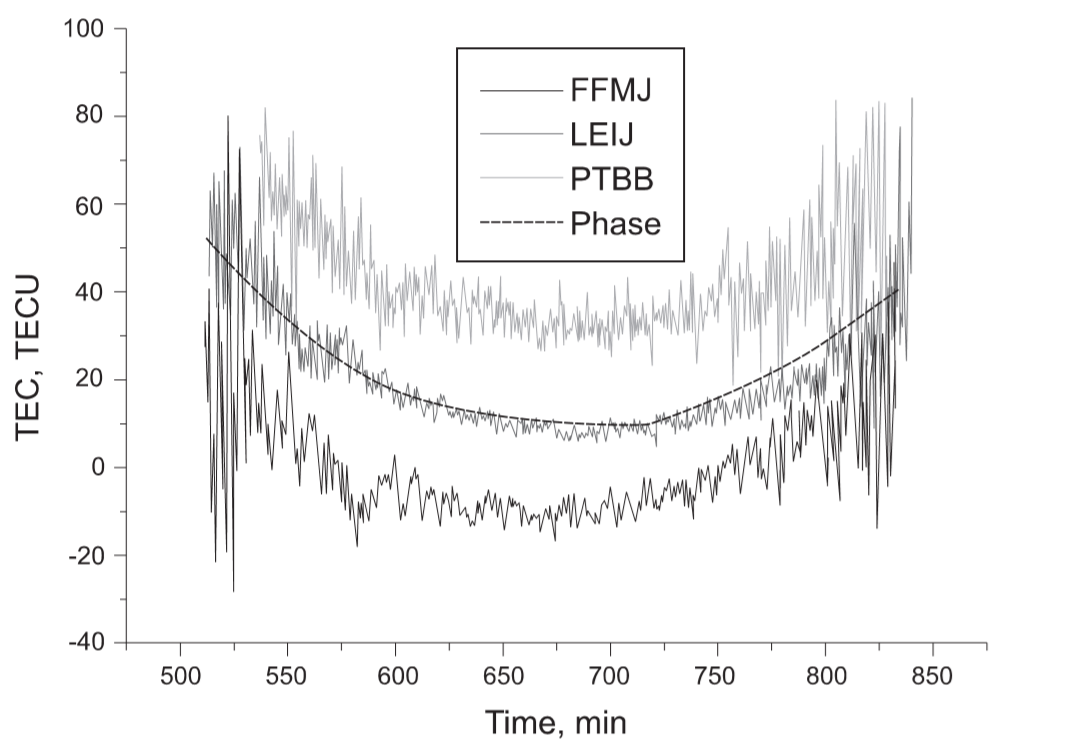
\includegraphics[width = 1\linewidth]{pics/pic2.png}
\caption{Зашумленность ПЭС, вычисленного по данным измерений группового (кривые <<FFMJ>>, <<LEIJ>> и <<PTBB>>) и фазового (кривая <<Phase>>) запаздывания сигналов GPS \cite{kozharin}.}
\label{pic2}
\end{figure}

Из-за высокого уровня шума в данных, определенных по кодовым задержкам, делает практически невозможным выделение вариаций ПЭС, обусловленными неоднородностями электронной концентрации в ионосфере. Таким образом, в ионосферных исследованиях предпочитают использовать ПЭС, измеренный фазовым методом. 

\subsubsection{Преобразование наклонного ПЭС  в вертикальное}
Измеренная по выше описанным формулам величина ПЭС пропорциональная расстоянию между спутником и приемником. В основном при исследовании ионосферных возмущений требуется некоторая нормировка амплитуда вариации ПЭС. С этой целью преобразуют полученные значения <<наклонного>> ПЭС в эквивалентное <<вертикальное>>, соответствующее углу места $\theta_S = 90^{\circ}$ 

Учитывая модель сферичной Земли, формула преобразования имеет вид \cite{klobuchar}:

\begin{equation}
I_V = I \cos{\left[ \arcsin{\left( \frac{R_E}{R_E + h_\text{max}} \cos{\theta_s}\right)} \right]},
\label{sfuntion}
\end{equation} 

где $I_V$ -- вертикальное значение ПЭС. 

\subsubsection{Дифференциальные кодовые задержки}
Стоит отметить, что при получении абсолютных значений полного электронного содержания, существует систематическая погрешность - ДКЗ (дифференциальная кодовая задержка). Появление ДКЗ связано с тем, что время прохождения сигналов диапазонов L1 и L2 в радиочастотных тактах приемника и спутника различается, и зависит от частоты сигнала.

ДКЗ определяется с помощью формулы:

\begin{equation}
I_{BIAS} = -\frac{f_1^2 f_2^2}{f_1^2 - f_2^2} \frac{1}{40.308} c\Delta \tau,
\end{equation}

где $I_{BIAS}$ - погрешность в ПЭС из-за влияния ДКЗ, $c$ - скорость света, $\Delta\tau$ - ДКЗ, $f_1$ и $f_2$ - первая и вторая частоты.

Также предполагается, что значение ДКЗ не изменяется в течение суток.


\newpage
\section{Исследовательская работа}
\subsection{Обработка данных со станций GNSS}
 GNSS станции записывают данные, получаемые со спутника, используя специальный формат записи RINEX (Receiver Independent Exchange Format).
 
 Существуют различные версии данного формата, каждый из которых поддерживает различные типы файлов: файл с данными наблюдений, файлы навигационного сообщения, файл с метеорологическими данными, файл с показаниями часов спутника и приемника.
 
 В рамках данной работы использовались файлы с данными наблюдений и навигационного сообщения. Из этих файлов доставалась информация об измерениях, предоставляемых спутниками, и данные о положении и движении спутников.
  
\begin{figure}[h!]
\centering
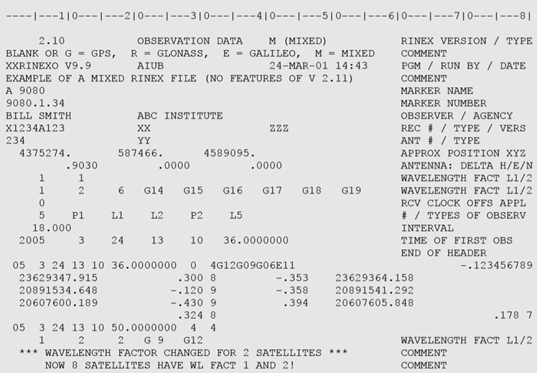
\includegraphics[width = 1\linewidth]{pics/rinex_obs.png}
\caption{Пример данных наблюдения для формата RINEX 2.1}
\end{figure}

\begin{figure}[h!]
\centering
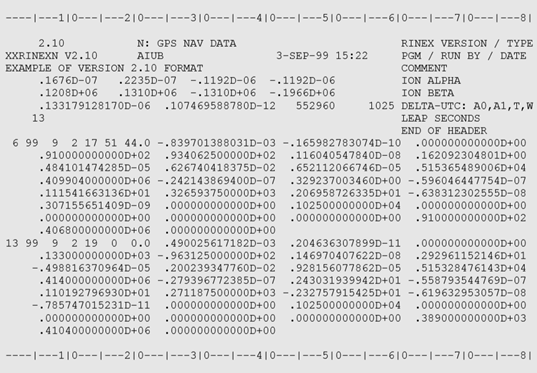
\includegraphics[width = 1\linewidth]{pics/rinex_nav.png}
\caption{Пример данных навигационного сообщения для формата RINEX 2.1}
\end{figure}


\newpage

\subsection{Вычисление наклонного ПЭС по групповым и фазовым измерениям}
После обработки данных со станций GNSS следующим шагом является вычисление наклонного значения ПЭС. Значение наклонного полного электронного содержания происходит с помощью формул (\ref{tecF}) и (\ref{tecP}), соответственно для фазового и кодового методов. 

Как упоминалось выше, из-за высокого уровня шума кодовых измерений практически невозможно выделить вариации ПЭС. Это обуславливает использование фазовых измерений для определения вариаций ПЭС, но начальное значение ПЭС остается неизвестным в силу существования фазовой неоднозначности.

Для решения этой проблемы используются кодовые измерения, с помощью которых находят неоднозначность фазы для фазовых измерений, так как они являются абсолютно с точностью до ошибки, обусловленной ДКЗ.

Измеренное значение ПЭС вычисляется по формуле:

\begin{equation}
I_{m} = I_{\varphi} + \frac{1}{N}\sum_{i=1}^N (I_p - I_{\varphi}),
\end{equation}

где $I_m$ - измеренное значение ПЭС с устраненной фазовой неоднозначностью, $I_\varphi$ - фазовые измерения, $I_p$ - кодовые измерения, $N$ - число измерений.  

\begin{figure}[h!]
\centering
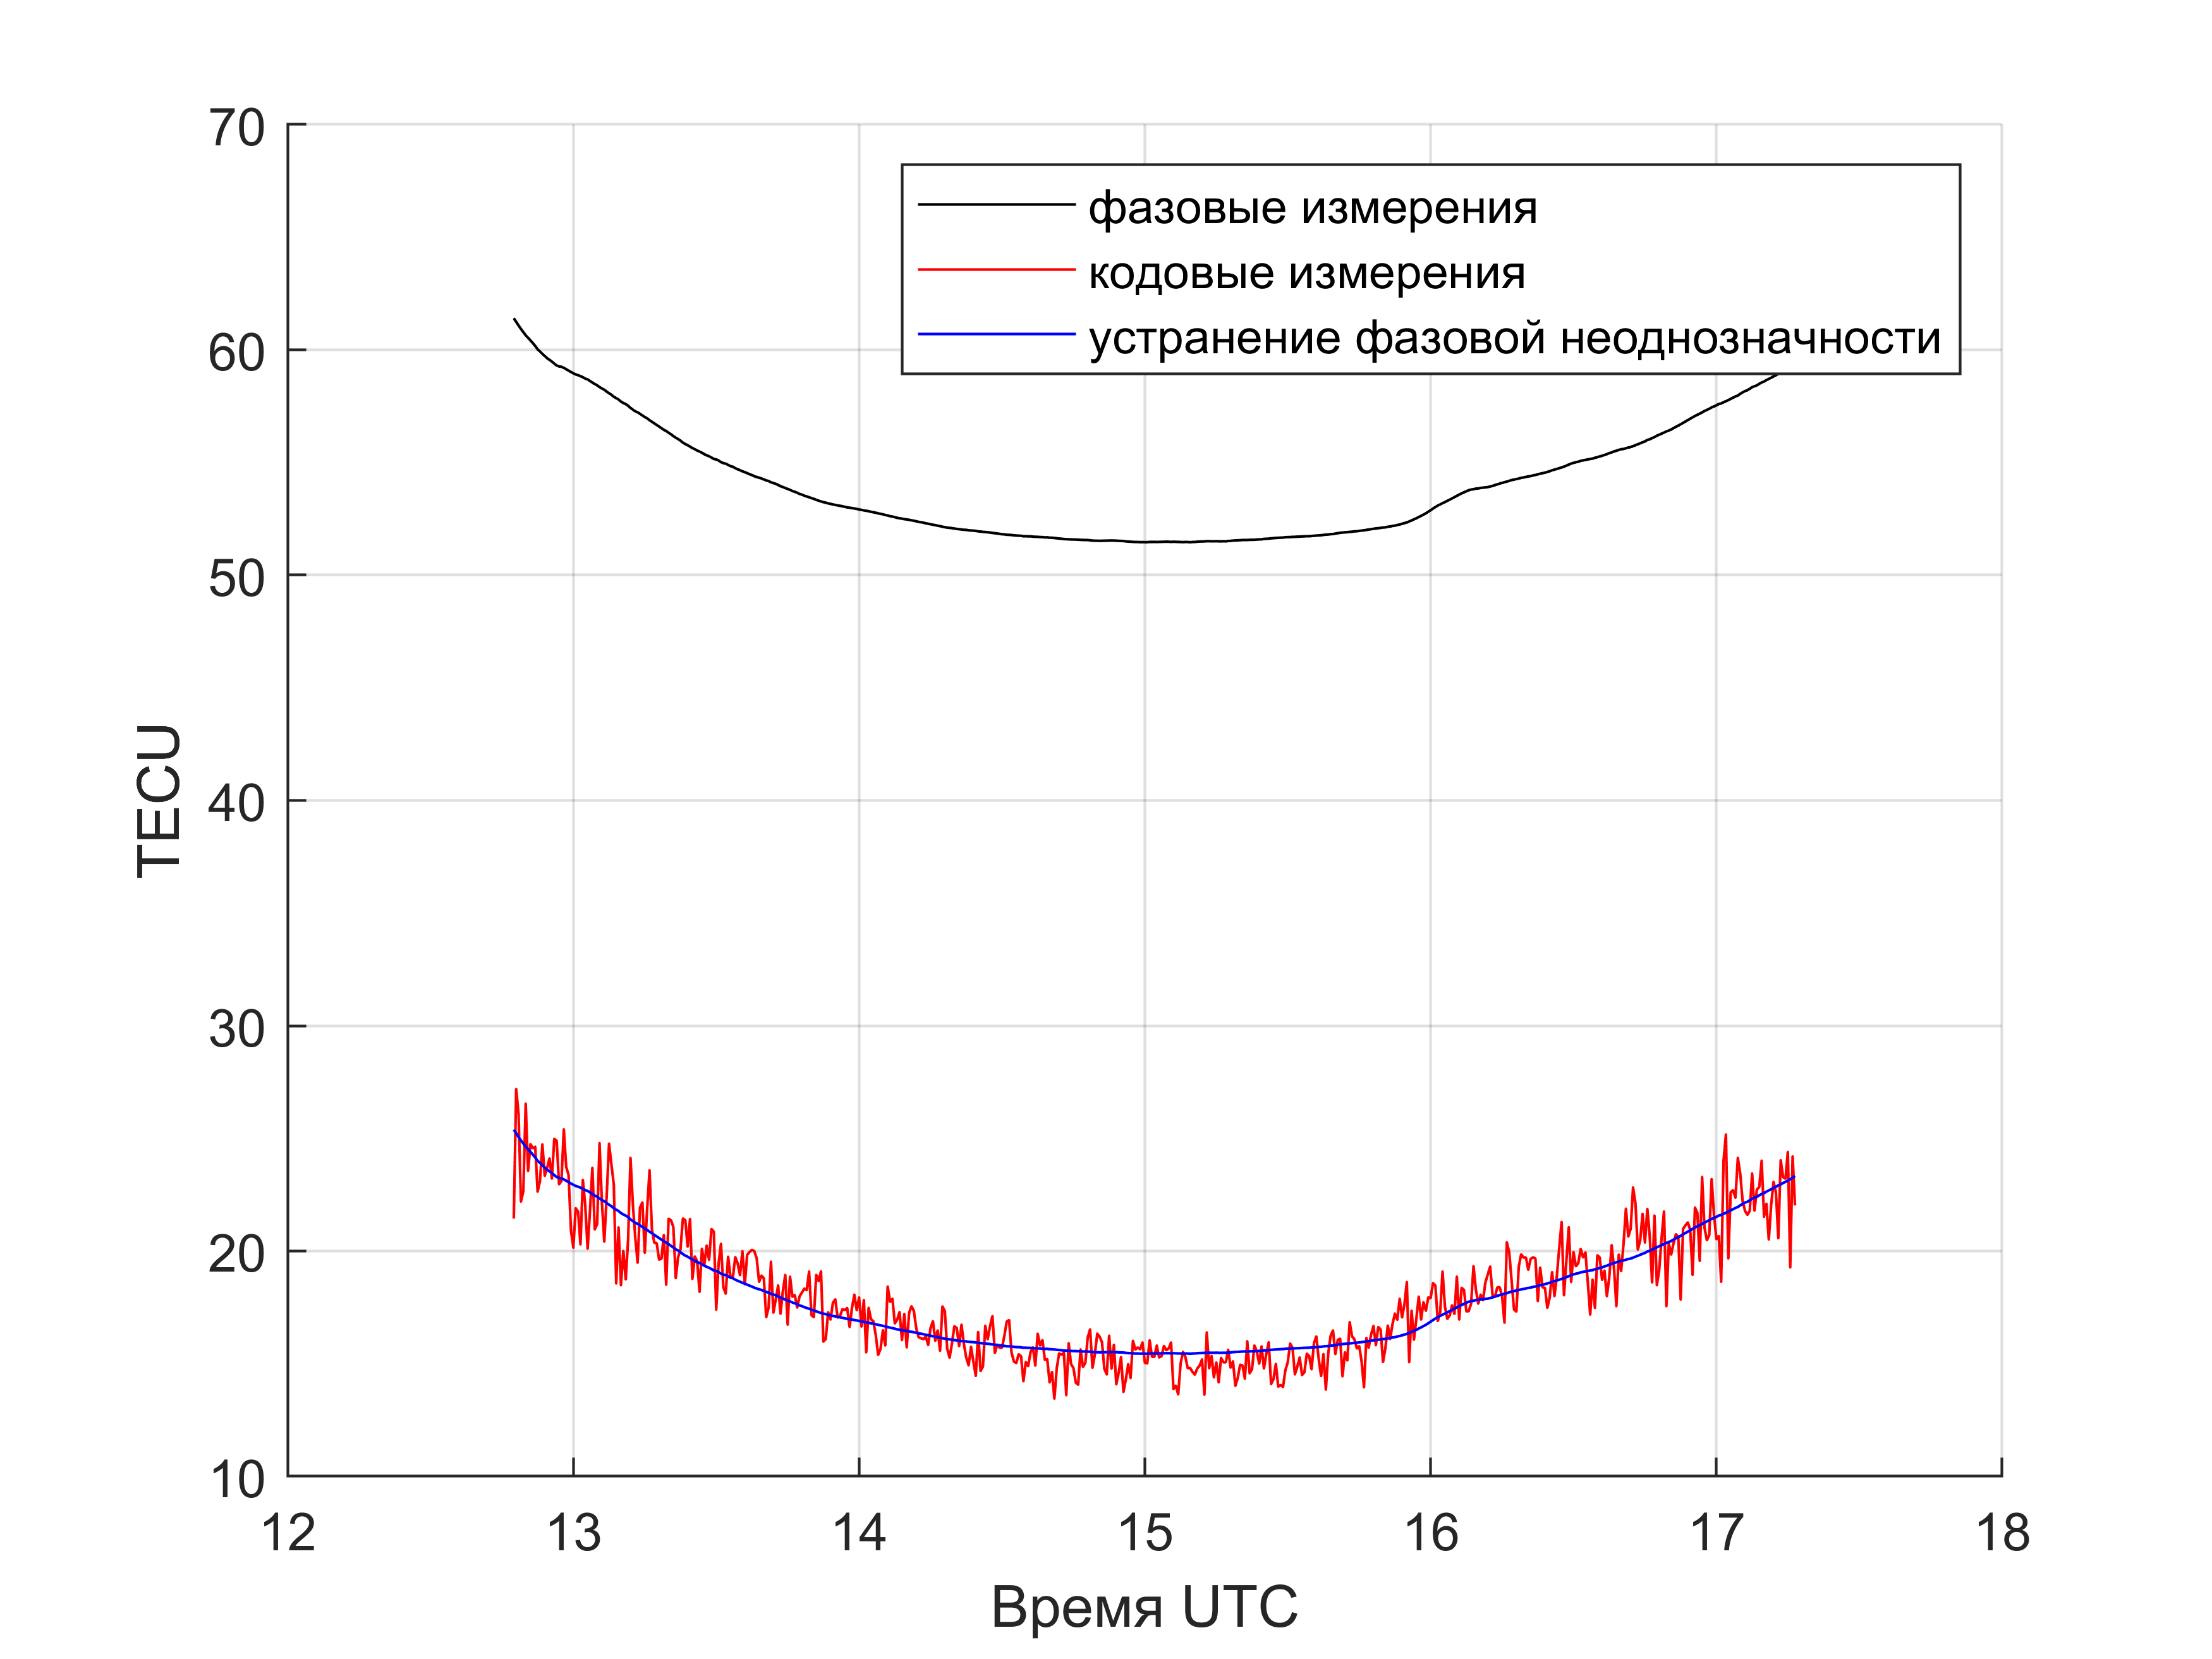
\includegraphics[width = 1\linewidth]{pics/clean_pics/stec.png}
\caption{Вычисленные значения ПЭС по кодовым и фазовым измерениям с учетом фазовой неоднозначности.}
\label{stecplot}
\end{figure}

Стоит отметить, что значения ПЭС, которые представлены на рисунке \ref{stecplot}, уже учитывают влияние дифференциальных кодовых задержек.

\newpage
\subsection{Оценка вертикального значения ПЭС}
Для вычисления вертикального значения полного электронного содержания используется модель, предложенная в работе Мыльниковой А.А. \cite{milnikova}.

Идея используемой модели заключается в том, что рассматривается разложение измеренного значения ПЭС в ряд Тейлора:

\begin{equation}
I_m = \frac{1}{S} \left[ I_v(\phi_0, l_0, t_0) + G_{\phi} \Delta\phi + G_l \Delta l + G_t \Delta t + ... \right] + I_{BIAS},
\label{taylor}
\end{equation}

где $I_m$ - измеренное значение наклонного ПЭС, $\Delta\phi$ - разница по широте между координатой ионосферной точки и станции $\phi_0$, $\Delta l$ - разница по долготе между координатой ионосферной точки и станции $l_0$, $\Delta t$ - разница между временем измерения и временем, для которого осуществляется расчет $t_0$, $G_{\phi} = \frac{\partial I_v}{\partial \phi}$, $G_l = \frac{\partial I_v}{\partial l}$, $G_t = \frac{\partial I_v}{\partial t}$ - пространственные и временная производные, $I_{BIAS}$ - ошибка, обусловленная ДКЗ, $S$ - функция преобразования (\ref{sfuntion}).

Для нахождения значений вертикального ПЭС строится система уравнений. Для каждого спутника записывается уравнение (\ref{taylor}) во все доступные моменты времени. Неизвестными величинами являются значение вертикального ПЭС, ДКЗ для каждого спутника, пространственные градиенты и временные производные. Расчет неизвестных осуществляется за полные сутки для выбранных моментов времени с интервалом, позволяющим использовать окрестность выбранных времен, в которой значение вертикального ПЭС принимается неизменным.

На рисунке \ref{solvedtec} представлены результаты решения системы уравнений для станции dent.

Верность данного решения можно подтвердить, сверив его с данными MADRIGAL\footnote{MADRIGAL - научная база данных о верхних слоях атмосферы.}. Видимые малые отклонения от проверочных данных связанны с тем, что координаты ионосферной точки над станцией dent не совпадают с координатами, которые предоставляет MADRIGAL, на величину не более 0.5 градусов.   

Также верность решения подтверждает сравнение дифференциальных кодовых задержек, полученных при решении системы уравнений, со значениями, которые публикует НАСА.

Для анализа ДКЗ спутников часто применяют условие нулевого среднего. Дифференциальные кодовые задержки для определенного спутника определяются как:

\begin{equation}
I_{BIAS\_SAT}^i = I_{BIAS}^i - \frac{\sum_{i=1}^{N}I_{BIAS}^i}{N}.
\end{equation}

где $N$ - число спутников, $I_{BIAS}^i$ - полученное значение ДКЗ из системы уравнений для $i$-го спутника.

\begin{figure}[h!]
\centering
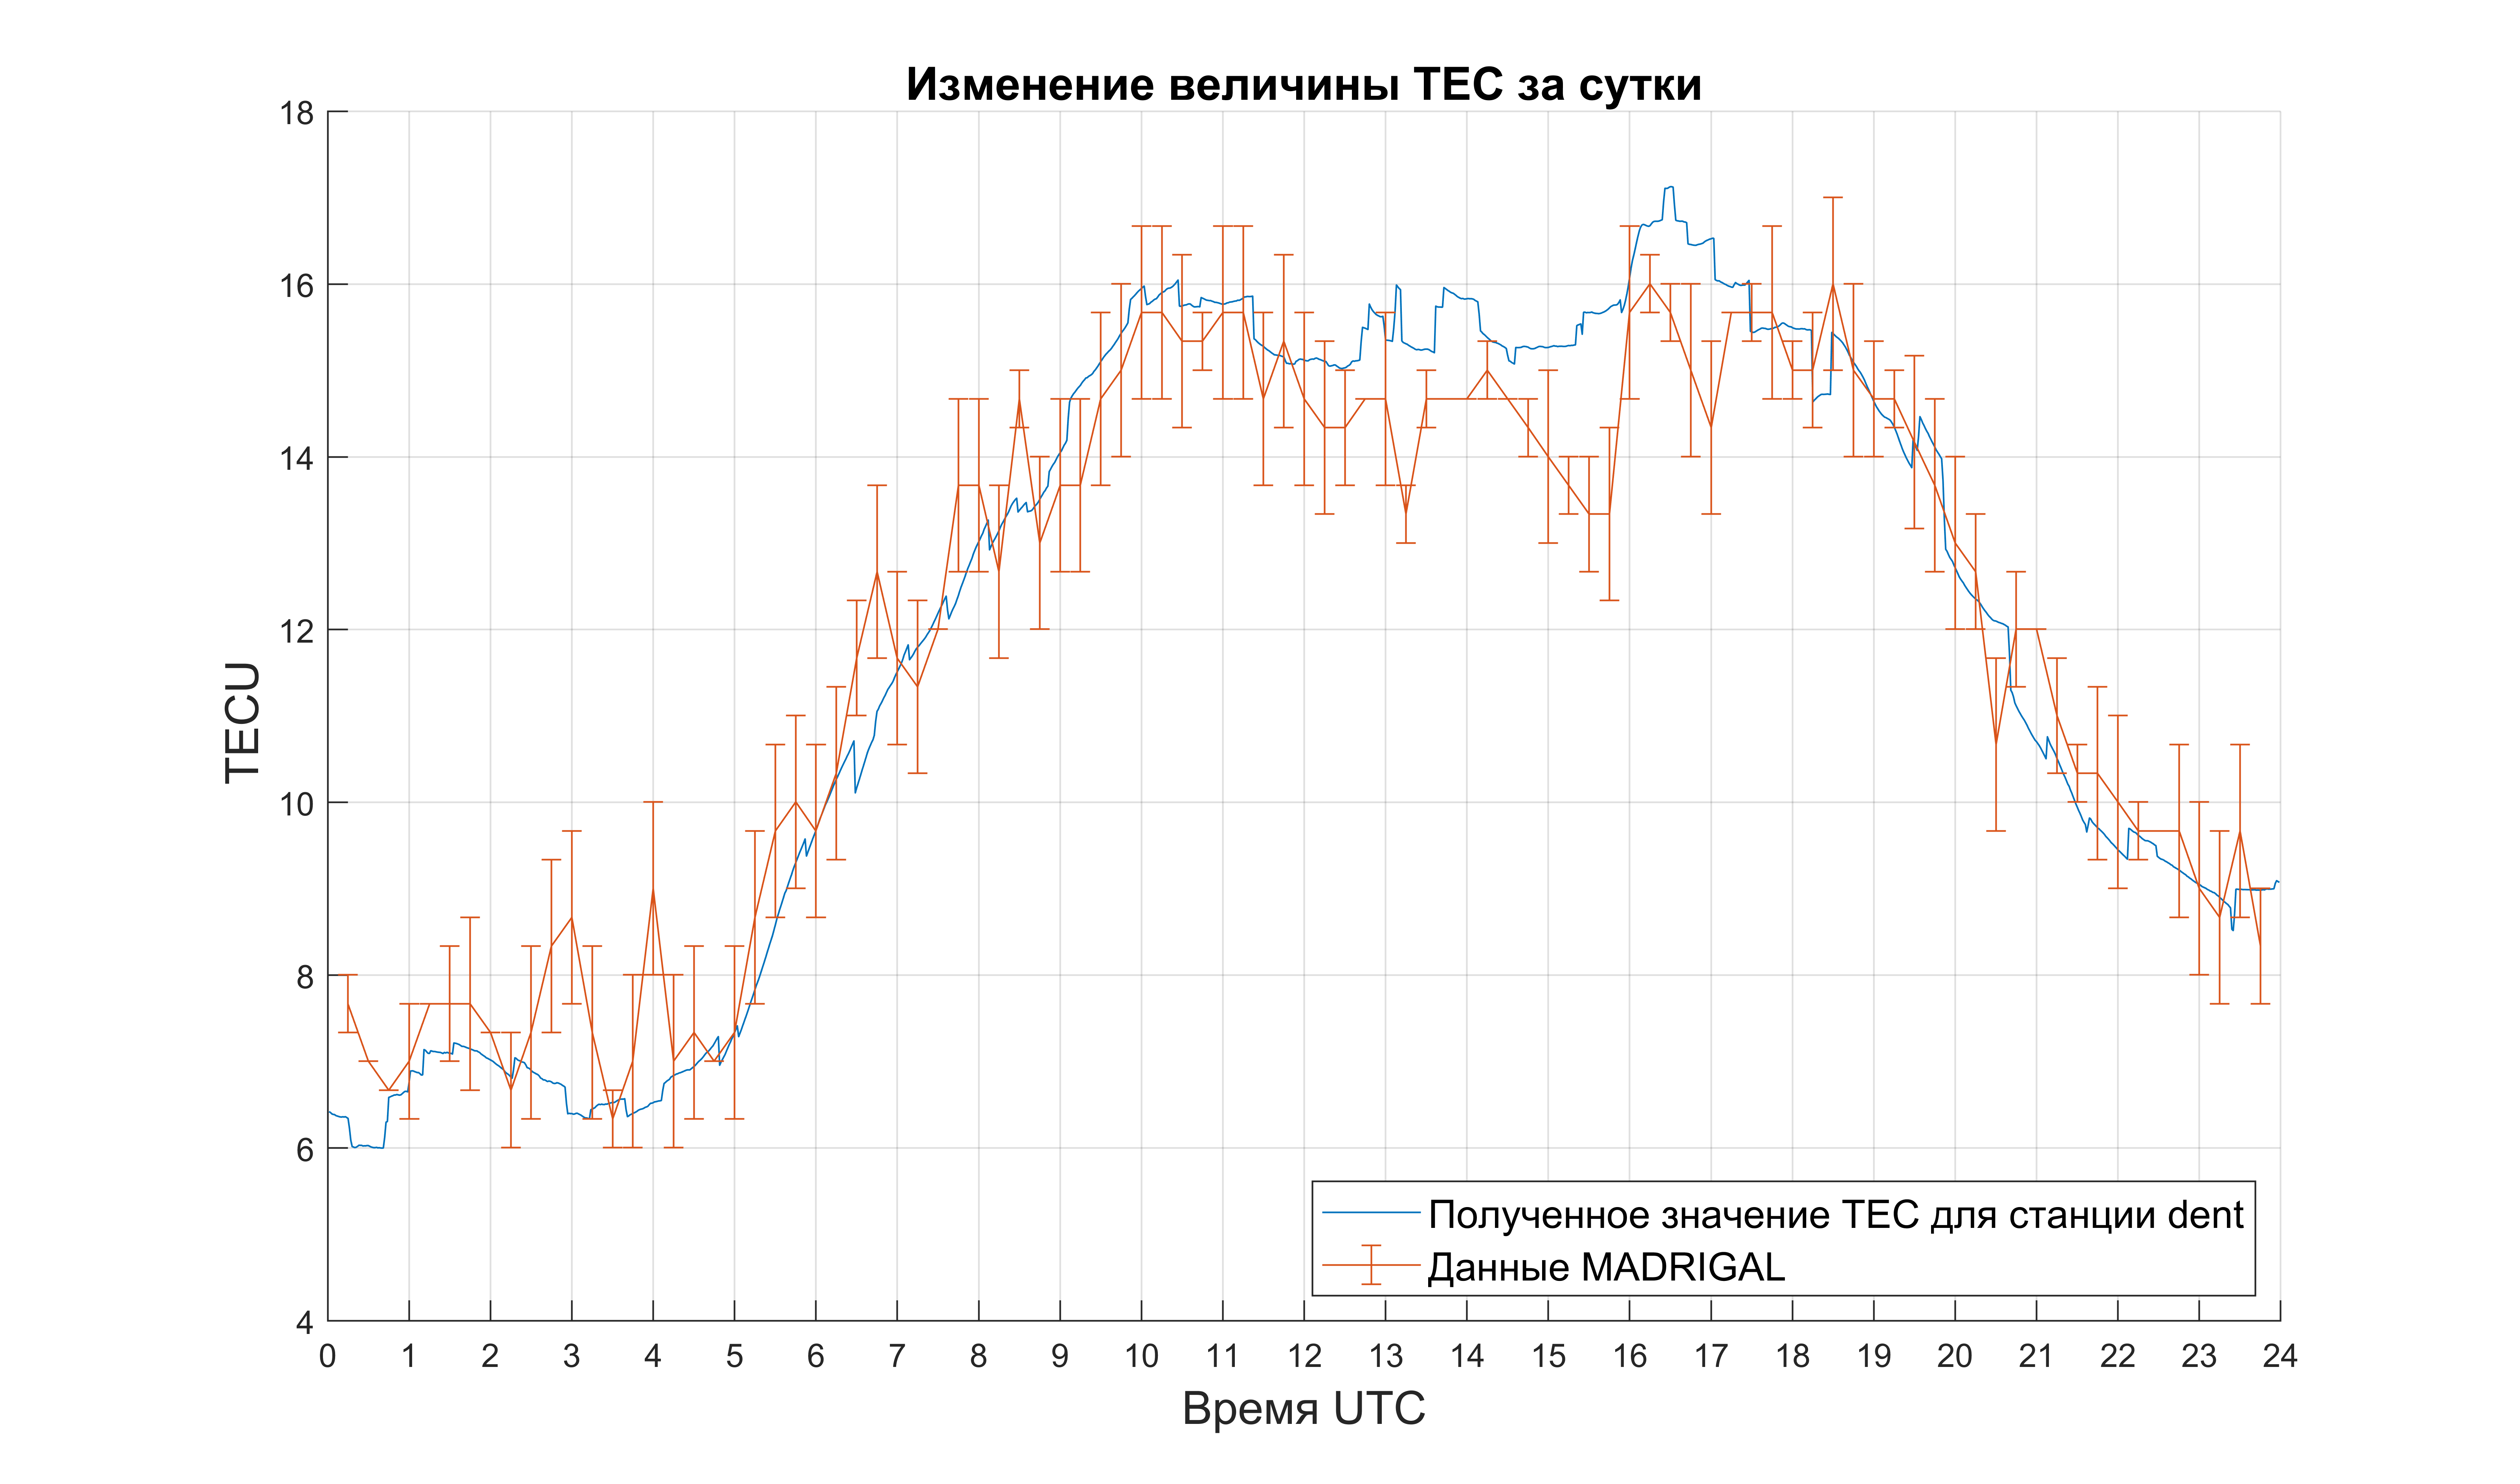
\includegraphics[width = 1\linewidth]{pics/clean_pics/tec_madrigal.png}
\caption{Значение вертикального ПЭС, полученное решением системы уравнений.}
\label{solvedtec}
\end{figure}


\subsection{Нахождение пространственных и временных зависимостей измерения ПЭС}
В рамках данной работы исследовалось поведение вариаций полного электронного содержания во время солнечной вспышки 10 сентября 2017 года. Данная вспышка имела класс активности X с индексом 9.8 баллов. Выброс произошел в районе 16 часов по UTC.

Для анализа влияния солнечной вспышки на ПЭС были выбраны станции, которые находились под освещением Солнца. Данные брались из открытых источников, а именно с сайта EUREF\footnote{Regional Reference Frame Sub-Commission for Europe.}.

Влияние солнечной вспышки можно оценить, сравнивая значение вычисленного ПЭС с изменением зенитного угла Солнца (Рисунок \ref{tecsun}). 

\begin{figure}[h]
\centering
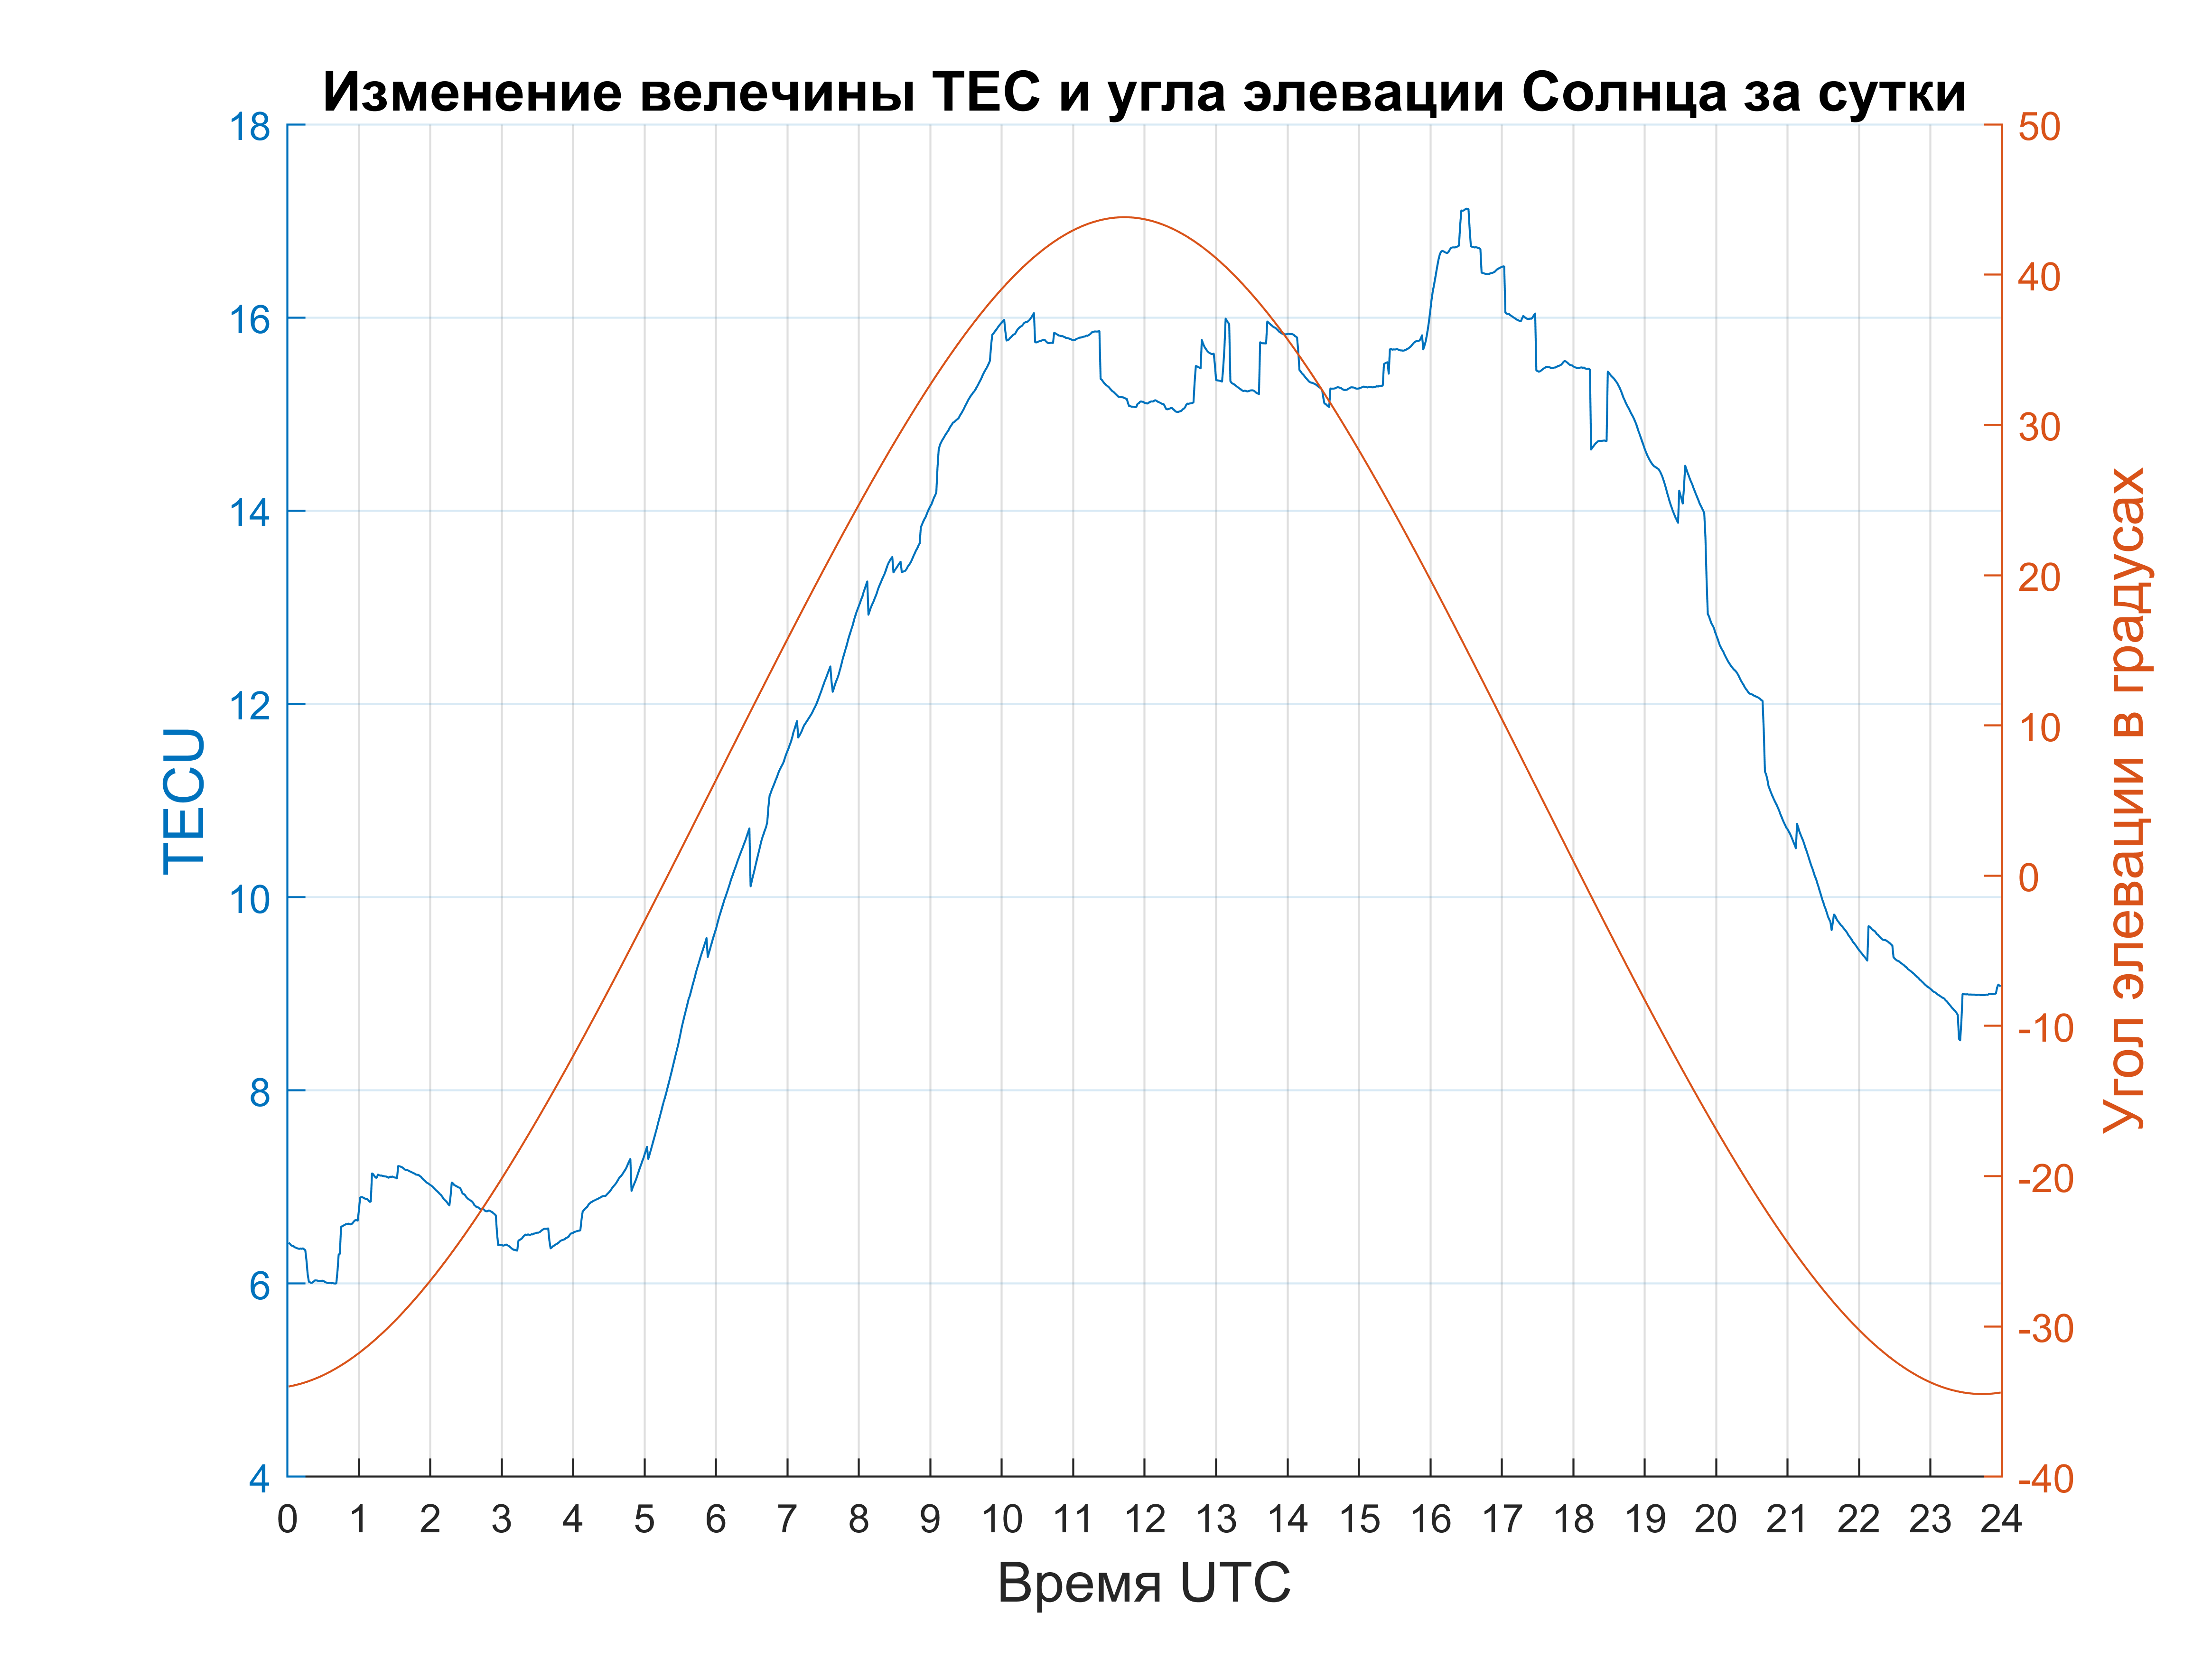
\includegraphics[width = 1\linewidth]{pics/clean_pics/tec_sun.png}
\caption{Зависимость полного электронного содержания от значения зенитного угла Солнца для станции dent}
\label{tecsun}
\end{figure} 

Данный график демонстрирует, что в начале дня значение полного электронного содержания изменяется пропорционально значению зенитного угла Солнца. Но в районе 16 часов эта пропорциональность смещается во времени из-за влияния солнечной вспышки. 

Далее предлагается рассмотреть значения ПЭС для станций, находящихся в Европе, чтобы найти пространственную зависимость изменения ПЭС, возникающую из-за солнечной вспышки. 

Для каждой из станций, с помощью описанного выше метода, было вычислено значение полного электронного содержания и его вариаций. На рисунке \ref{dtec15} показаны значения производной ПЭС для некоторых станций во время солнечной вспышки.

\begin{landscape}
\begin{figure}[h!]
\centering
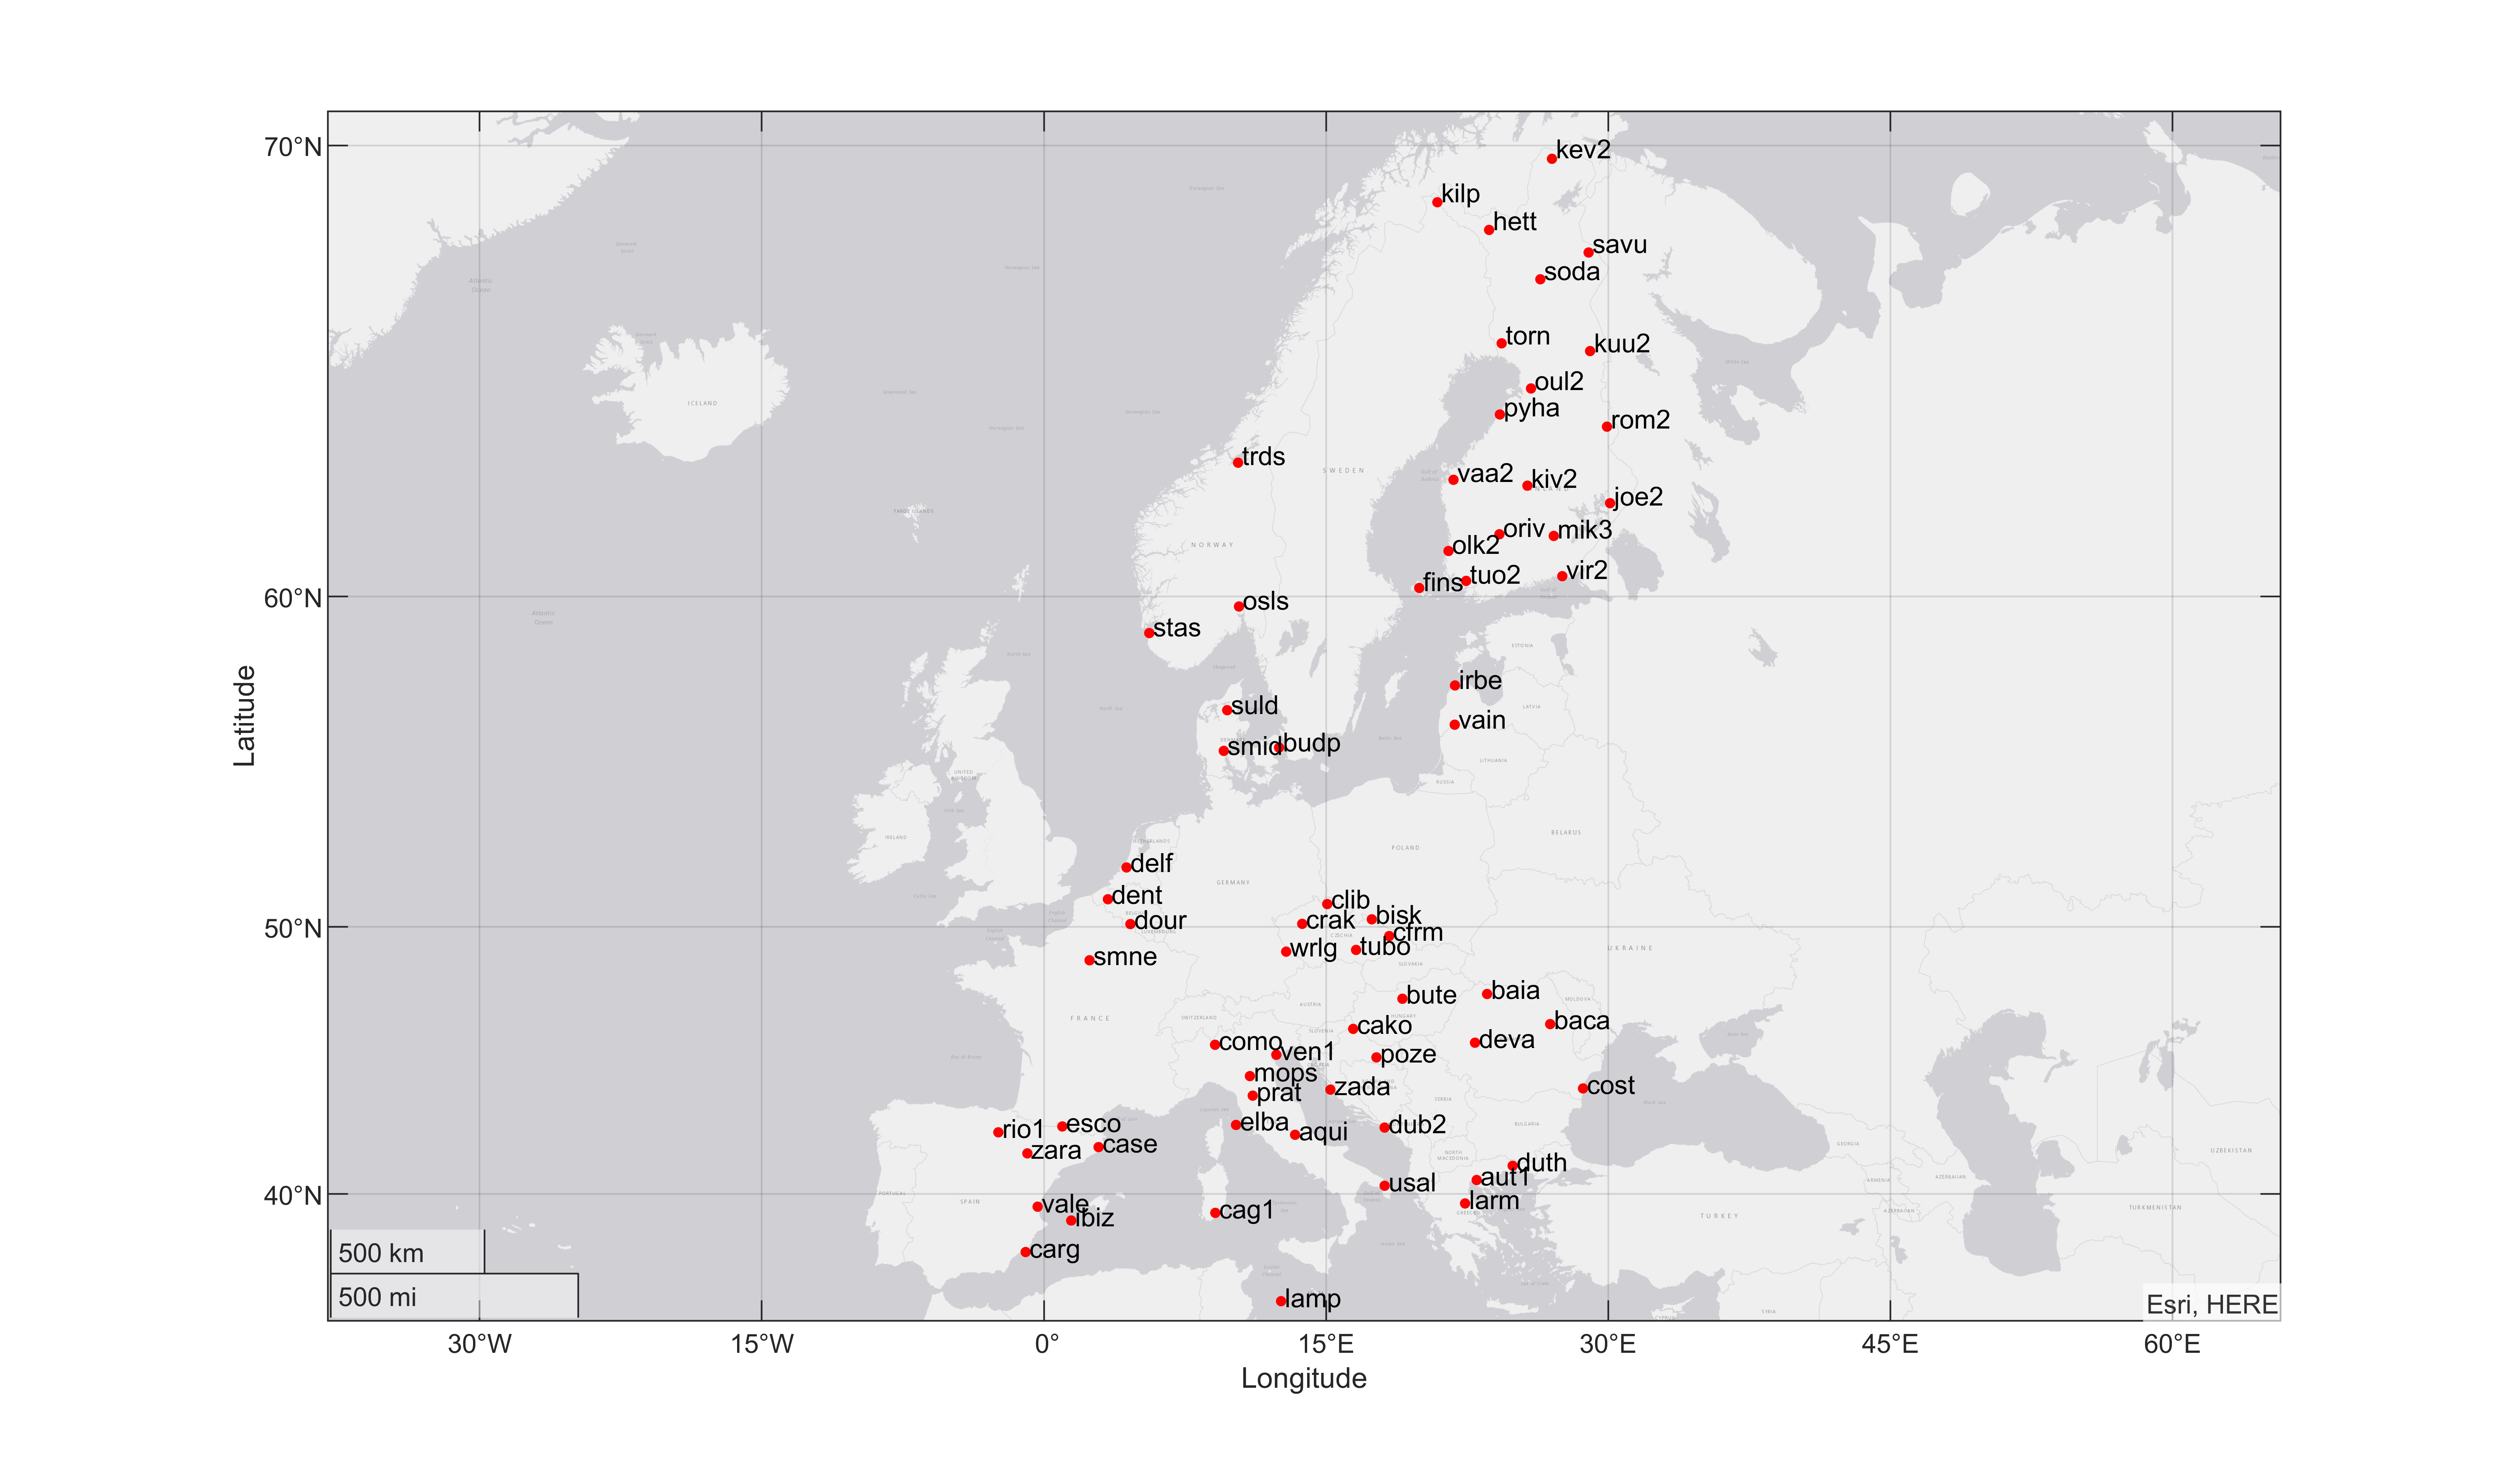
\includegraphics[width = 1\linewidth]{pics/clean_pics/stations.png}
\caption{Расположение выбранных станций.}
\end{figure}
\end{landscape}



\begin{landscape}
\begin{figure}[h!]
\centering
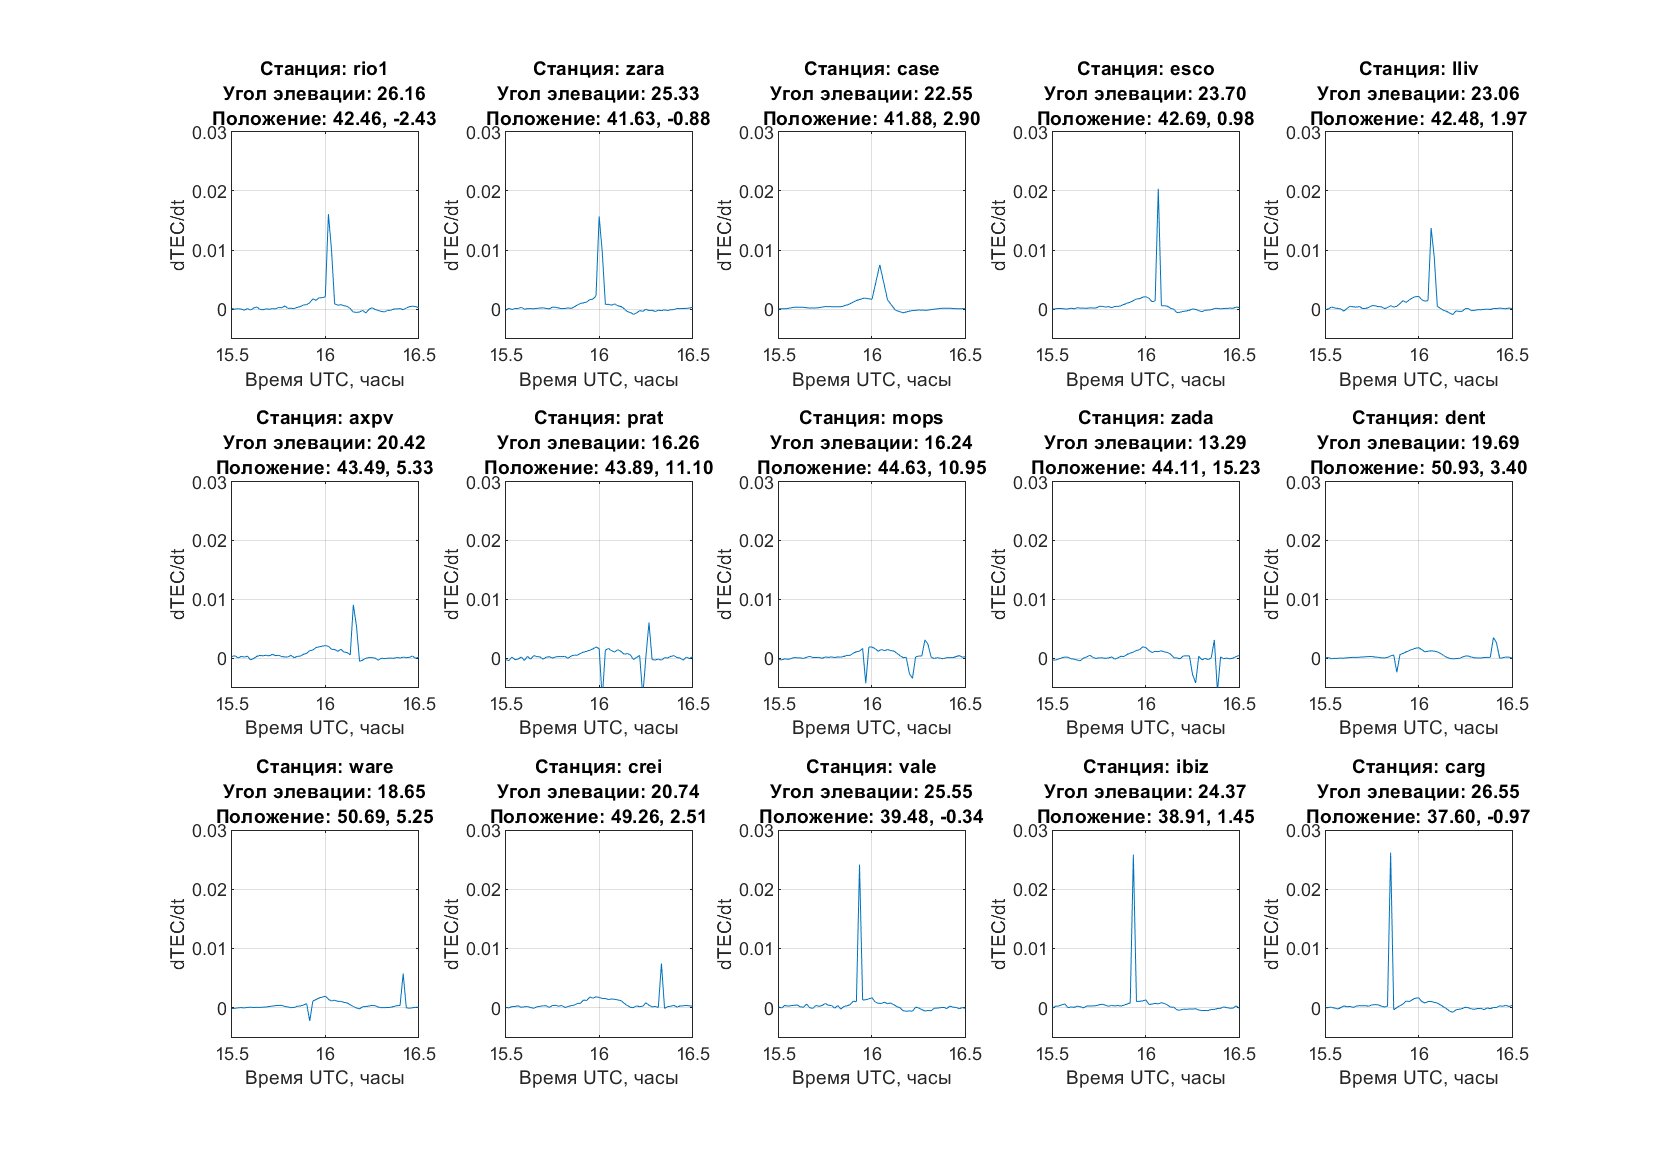
\includegraphics[width = 0.85\linewidth]{pics/clean_pics/dtec15.png}
\caption{Зависимость временной производной ПЭС во время солнечной вспышки для станций с различным зенитным углом Солнца.}
\label{dtec15}
\end{figure}
\end{landscape}

На рисунке \ref{dtecsun} приведены пиковые значения временной производной полного электронного содержания для всех выбранных станций.

Полученные значения производных зависят от зенитного угла Солнца. Это и логично, ведь чем выше находится Солнце, тем более сильно освещена данная территория, и влияние вспышки имеет наибольшее воздействие на состояние ионосферы.

\begin{figure}[h!]
\centering
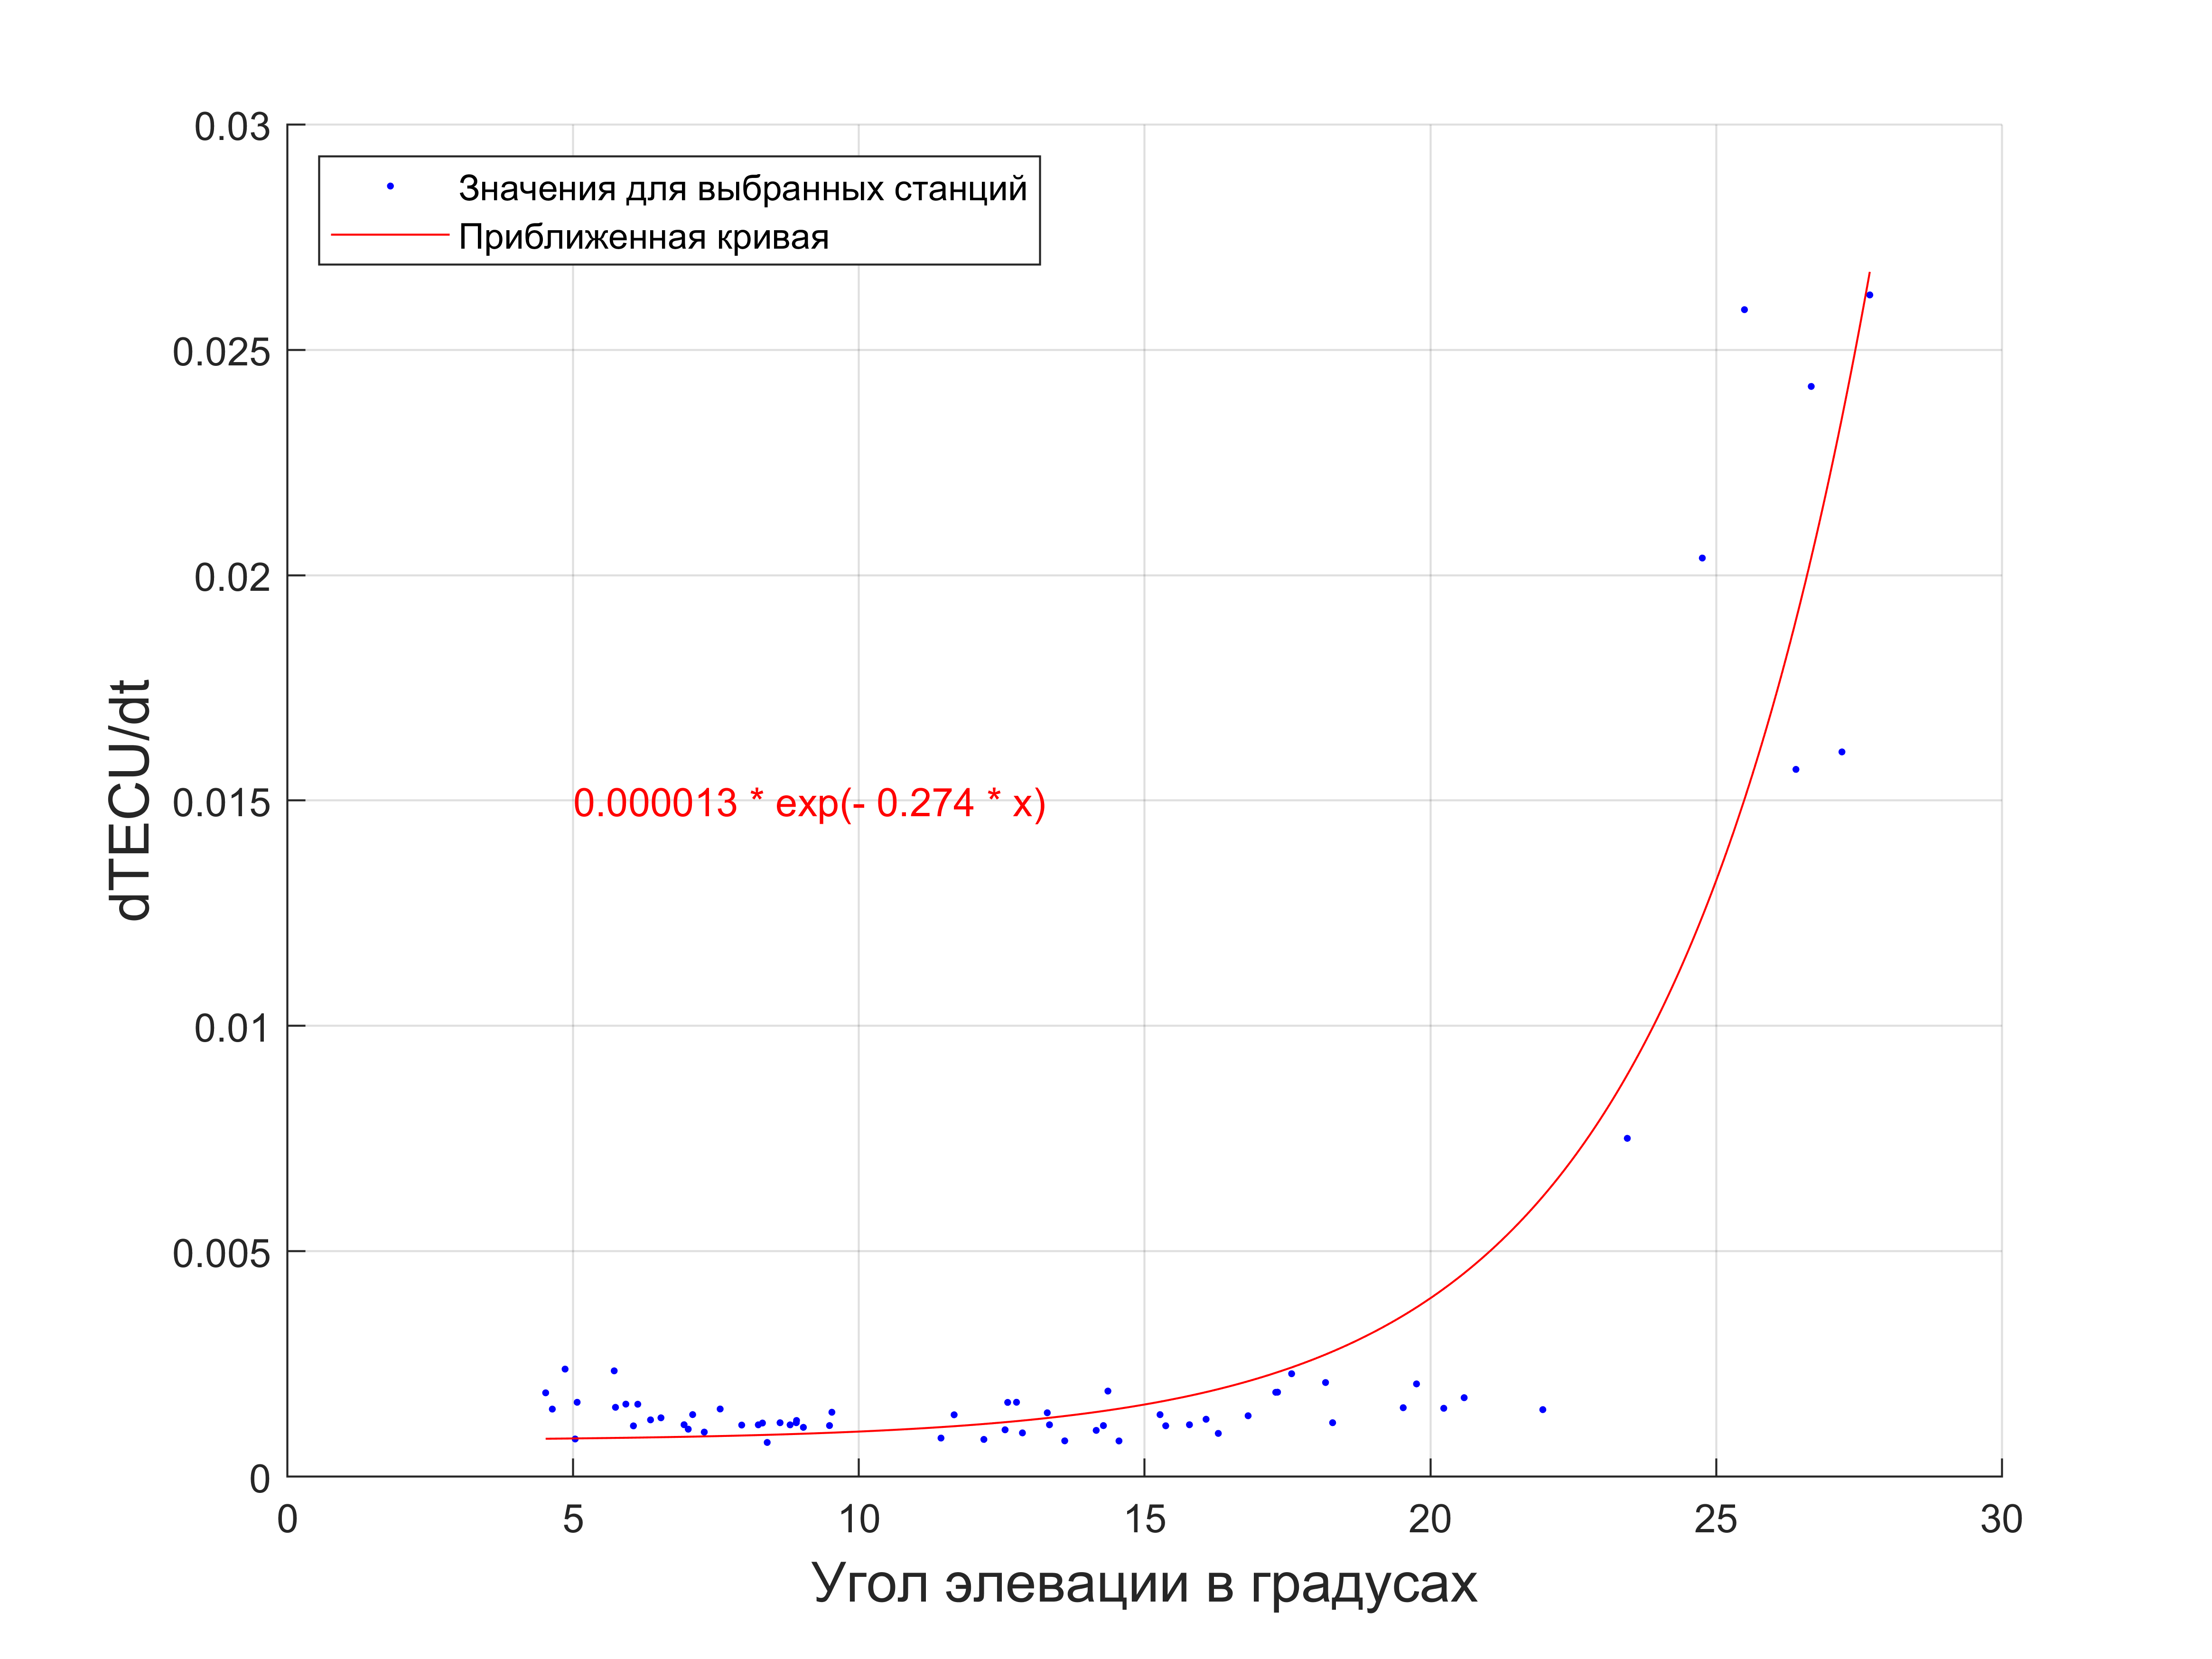
\includegraphics[width = 1\linewidth]{pics/clean_pics/dtec_elev.png}
\caption{Зависимость пикового значения временной производной ПЭС от угла возвышения Солнца во время солнечной вспышки.}
\label{dtecsun}
\end{figure}

Также можно рассмотреть изменение пикового значения производной в зависимости от изменения координаты широты или долготы. На рисунках \ref{dteclat} и \ref{dteclon} приведены результаты для выбранных станций.


\begin{figure}[H]
\centering
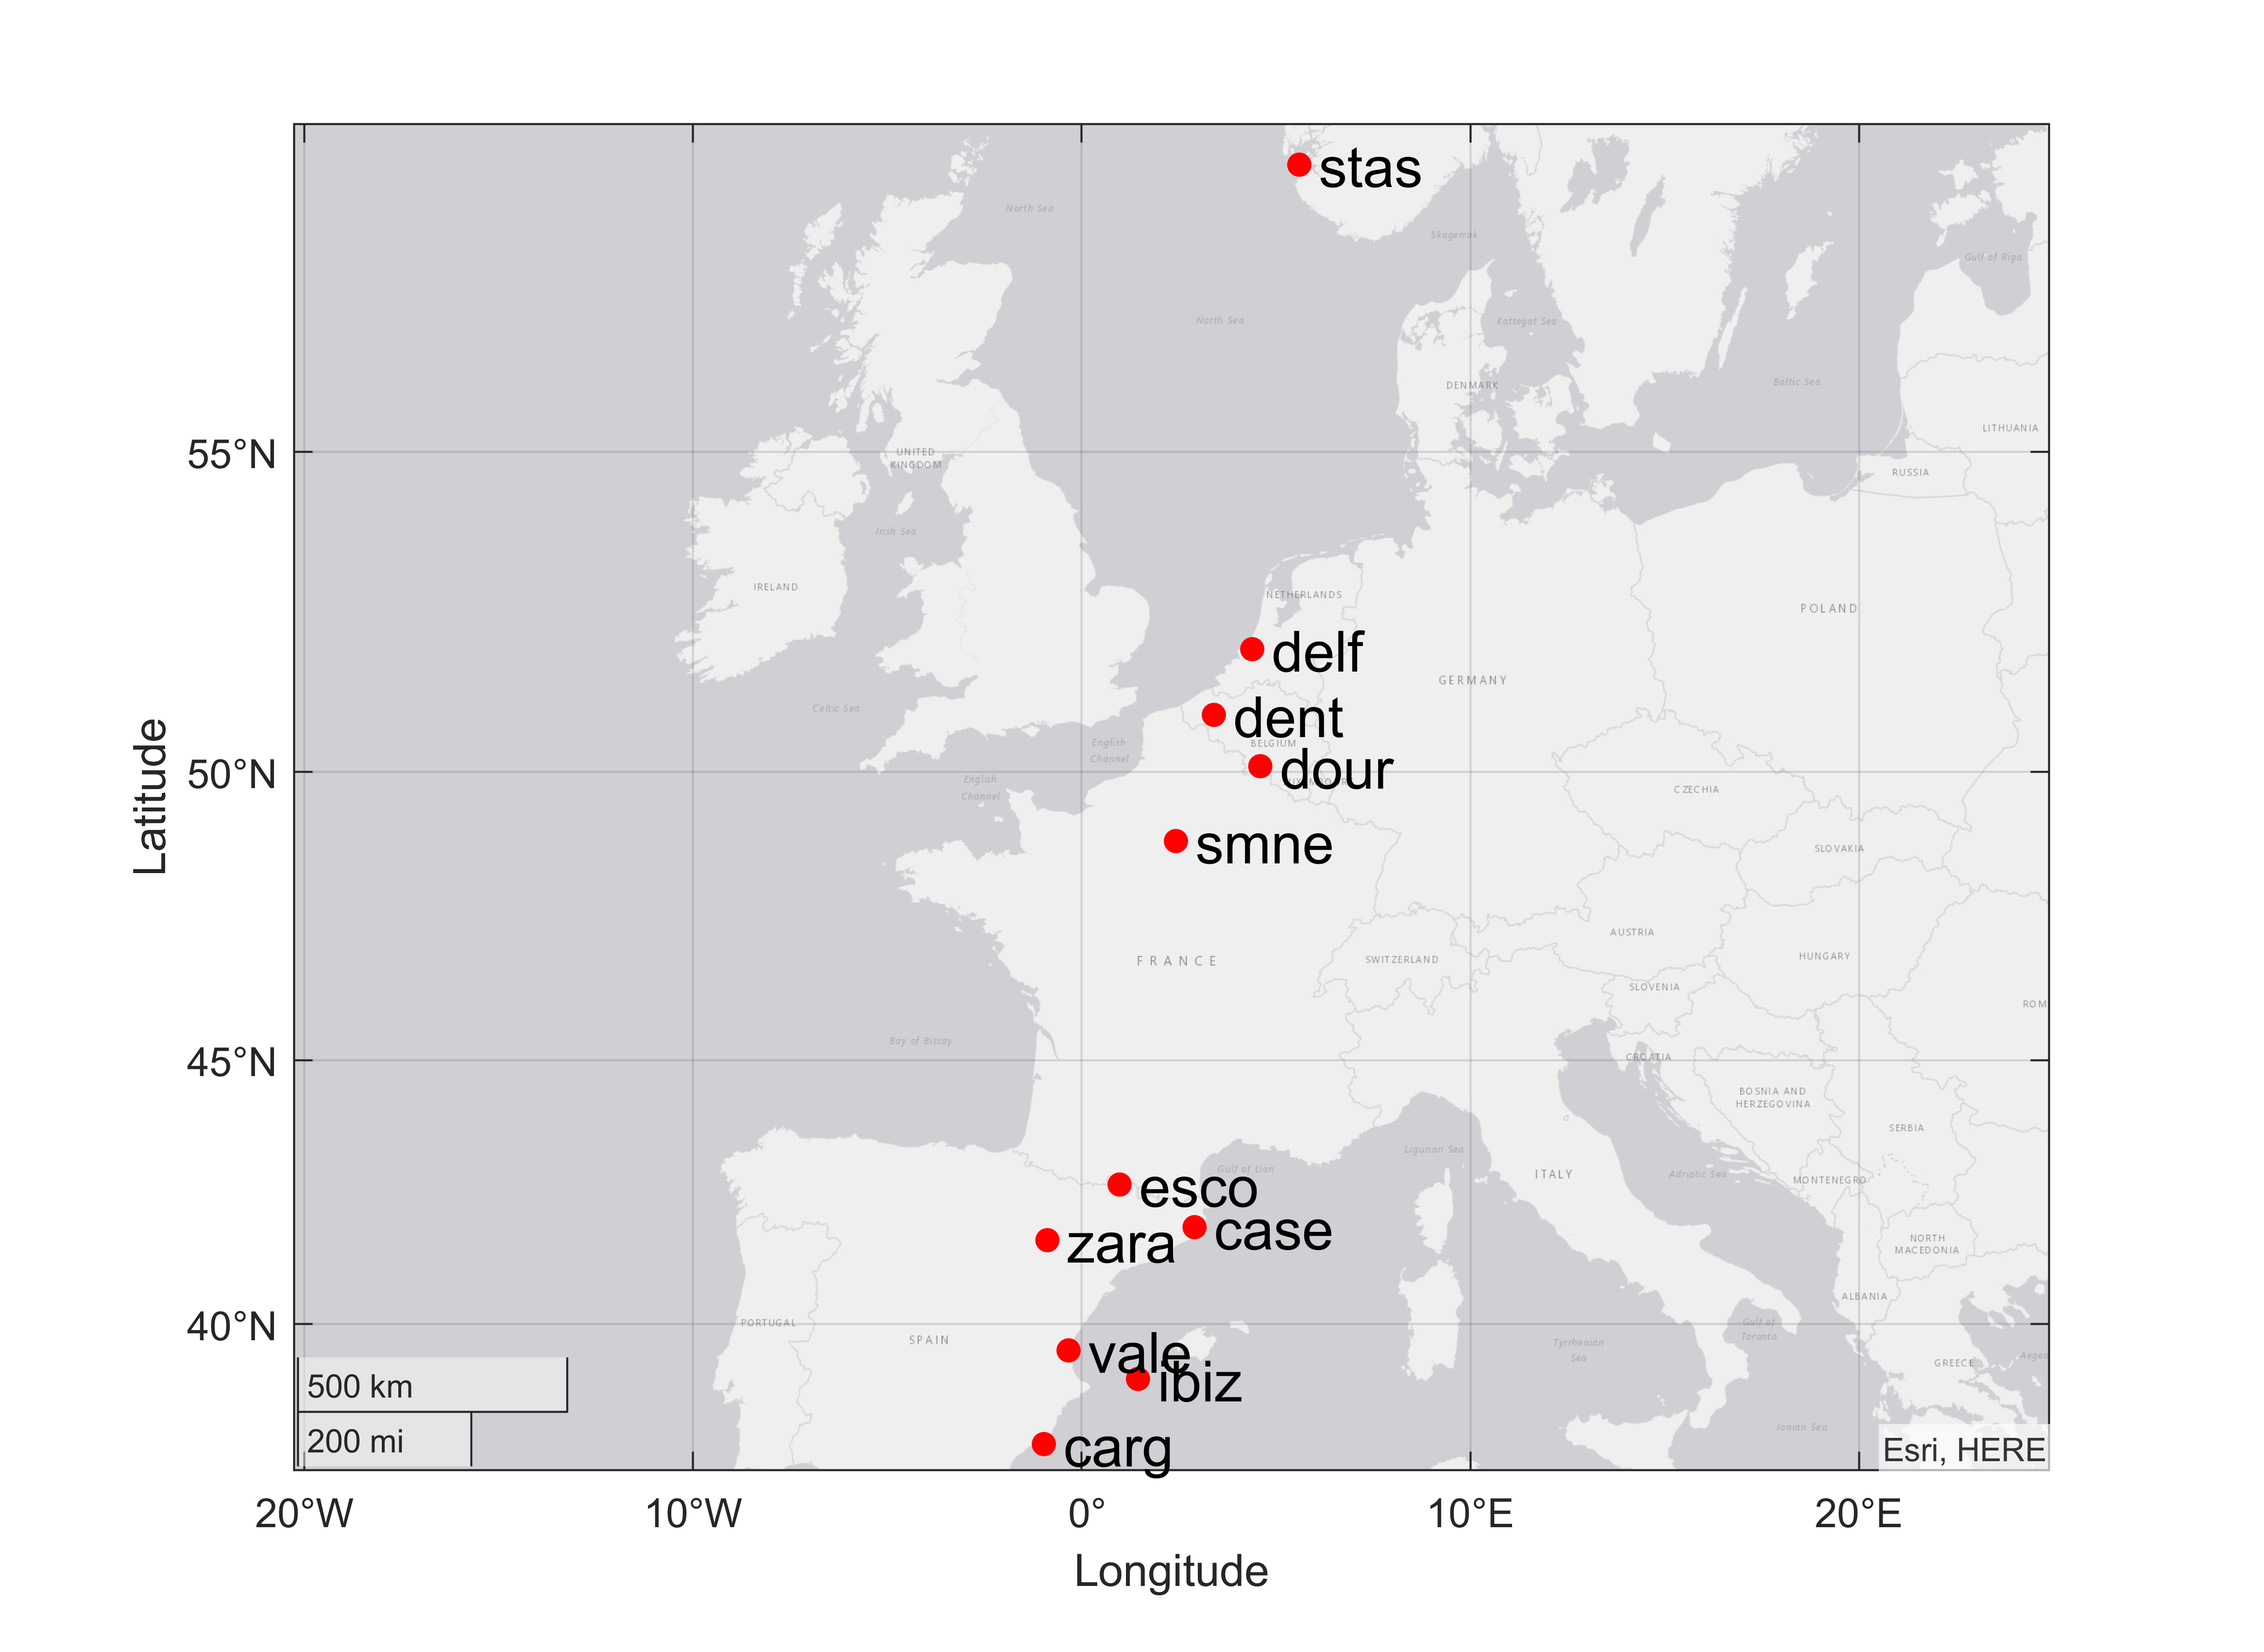
\includegraphics[width = 1\linewidth]{pics/clean_pics/latStations.png}
\caption{Выбранные станция для широты}
\label{stationslat}
\end{figure}

\begin{figure}[H]
\centering
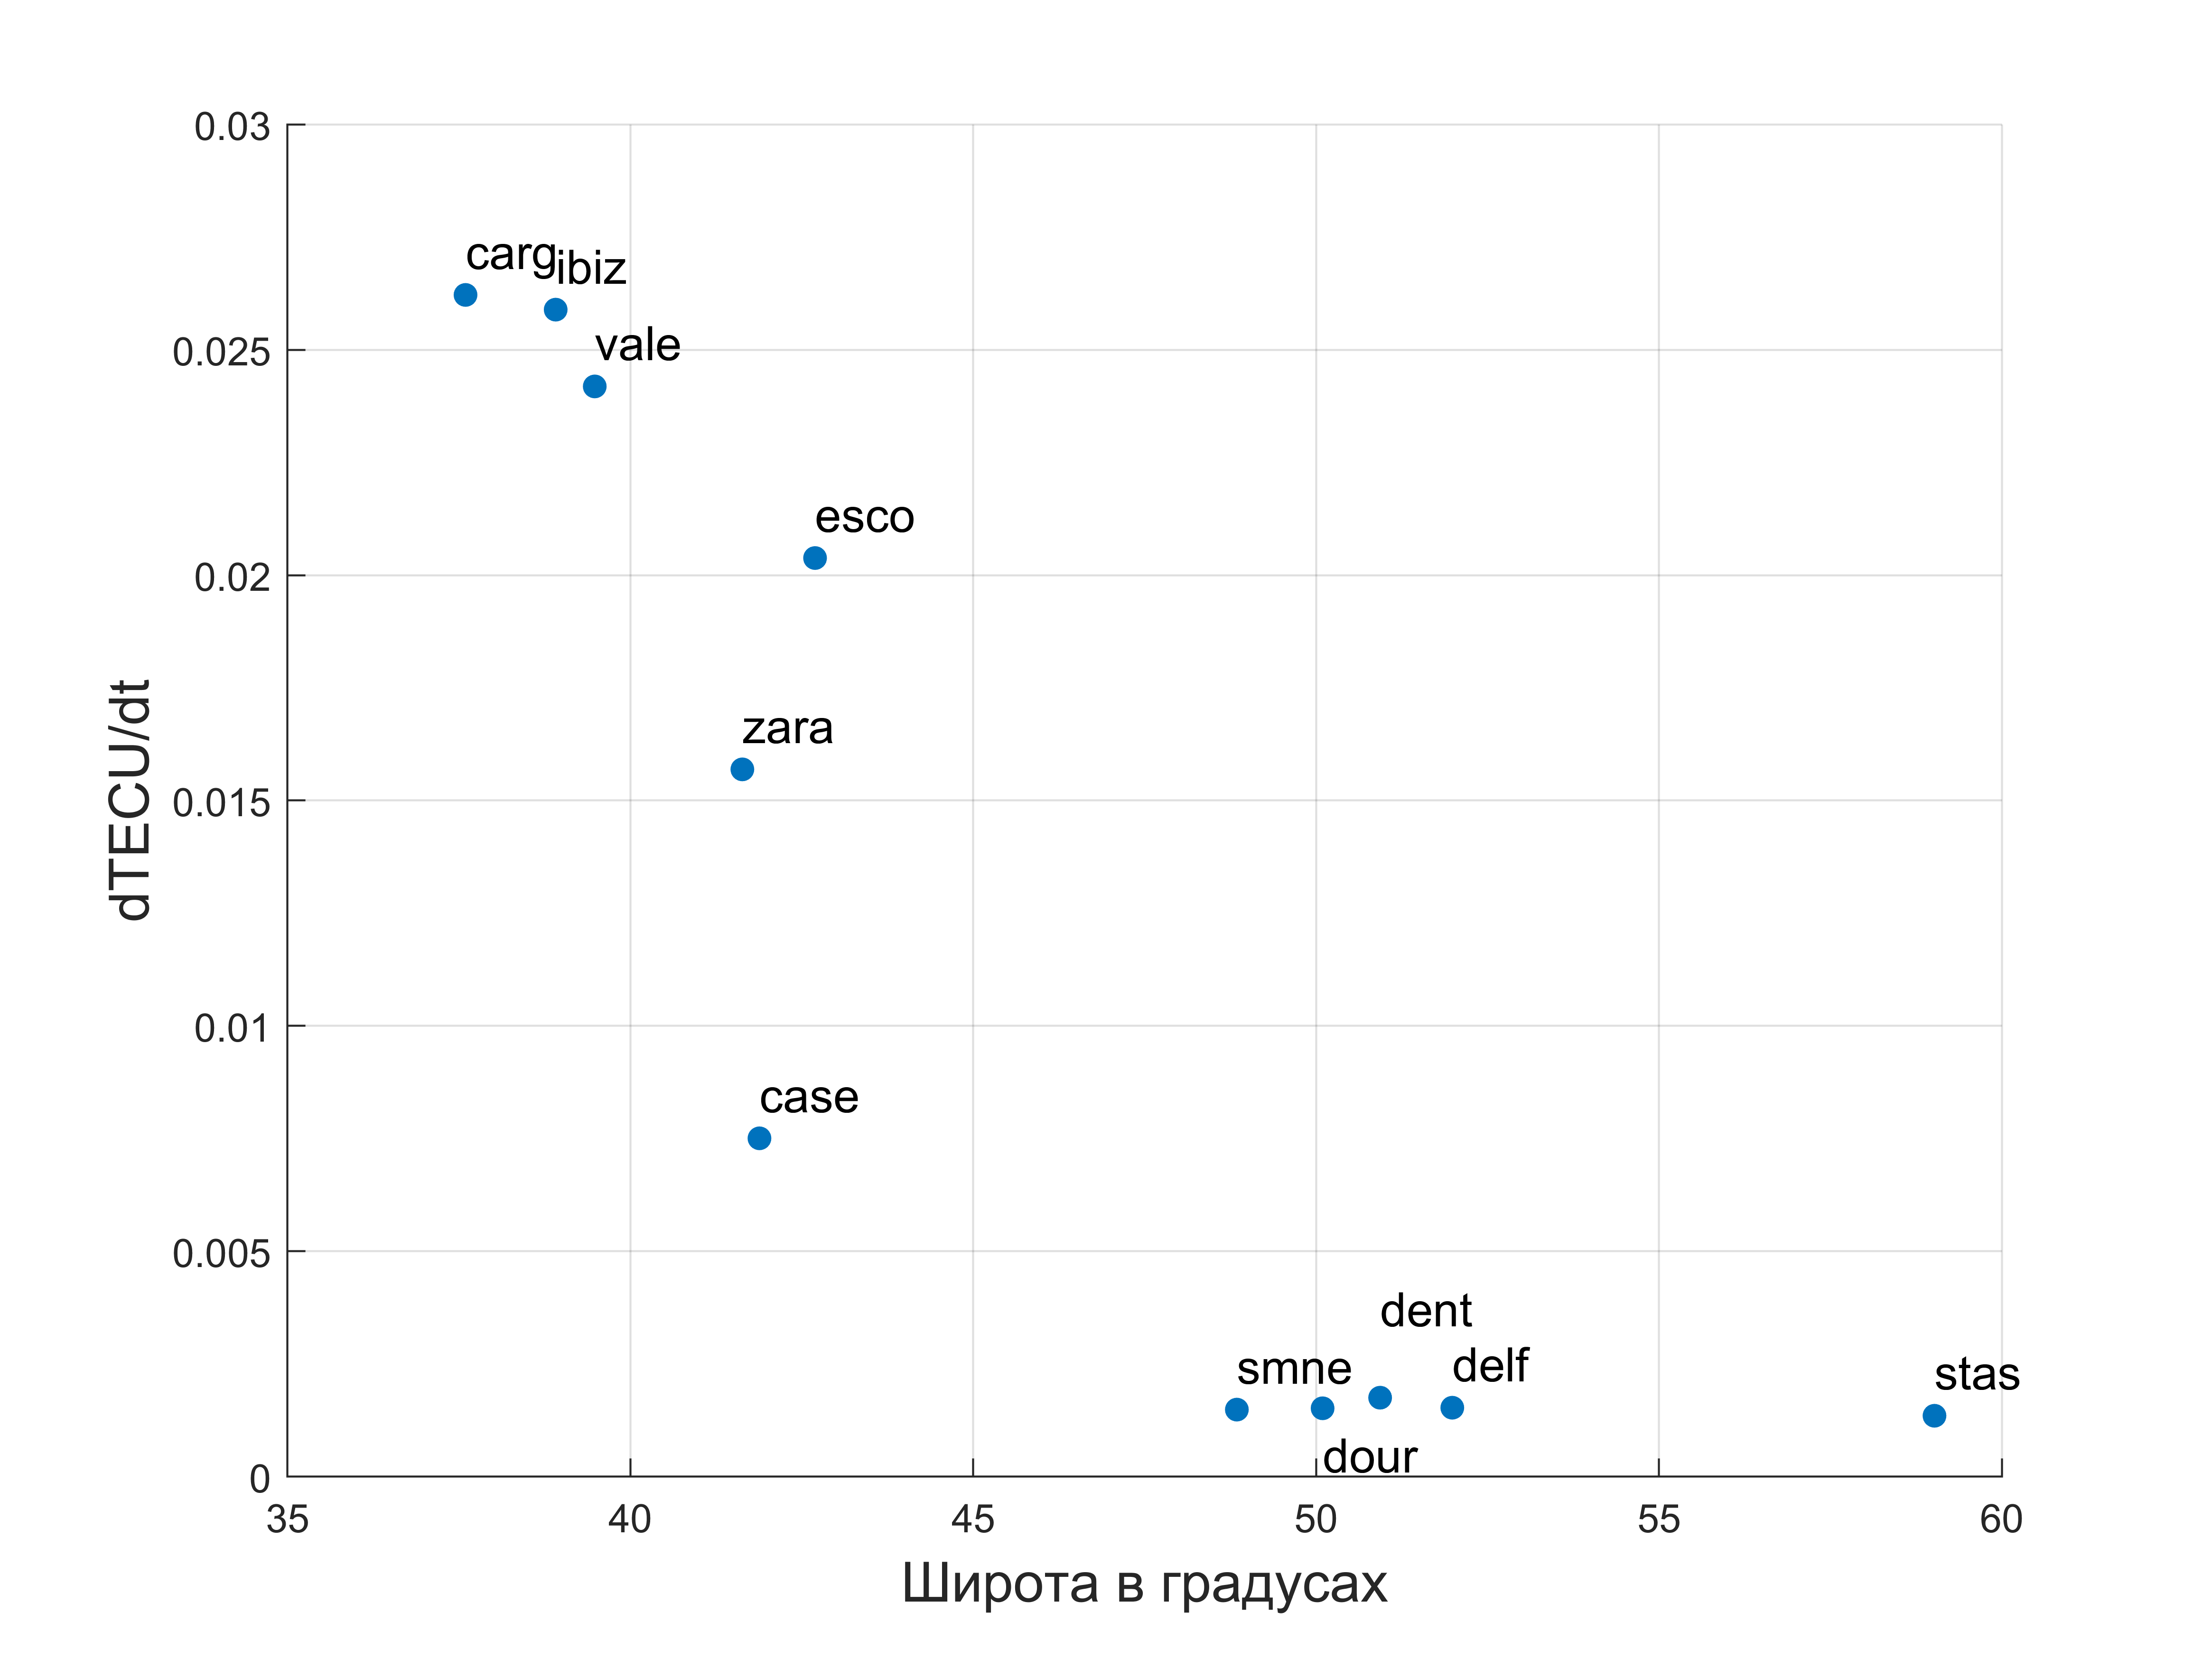
\includegraphics[width = 1\linewidth]{pics/clean_pics/dtec_lat.png}
\caption{Зависимость пикового значения временной производной от изменения координаты широты.}
\label{dteclat}
\end{figure}

\begin{figure}[H]
\centering
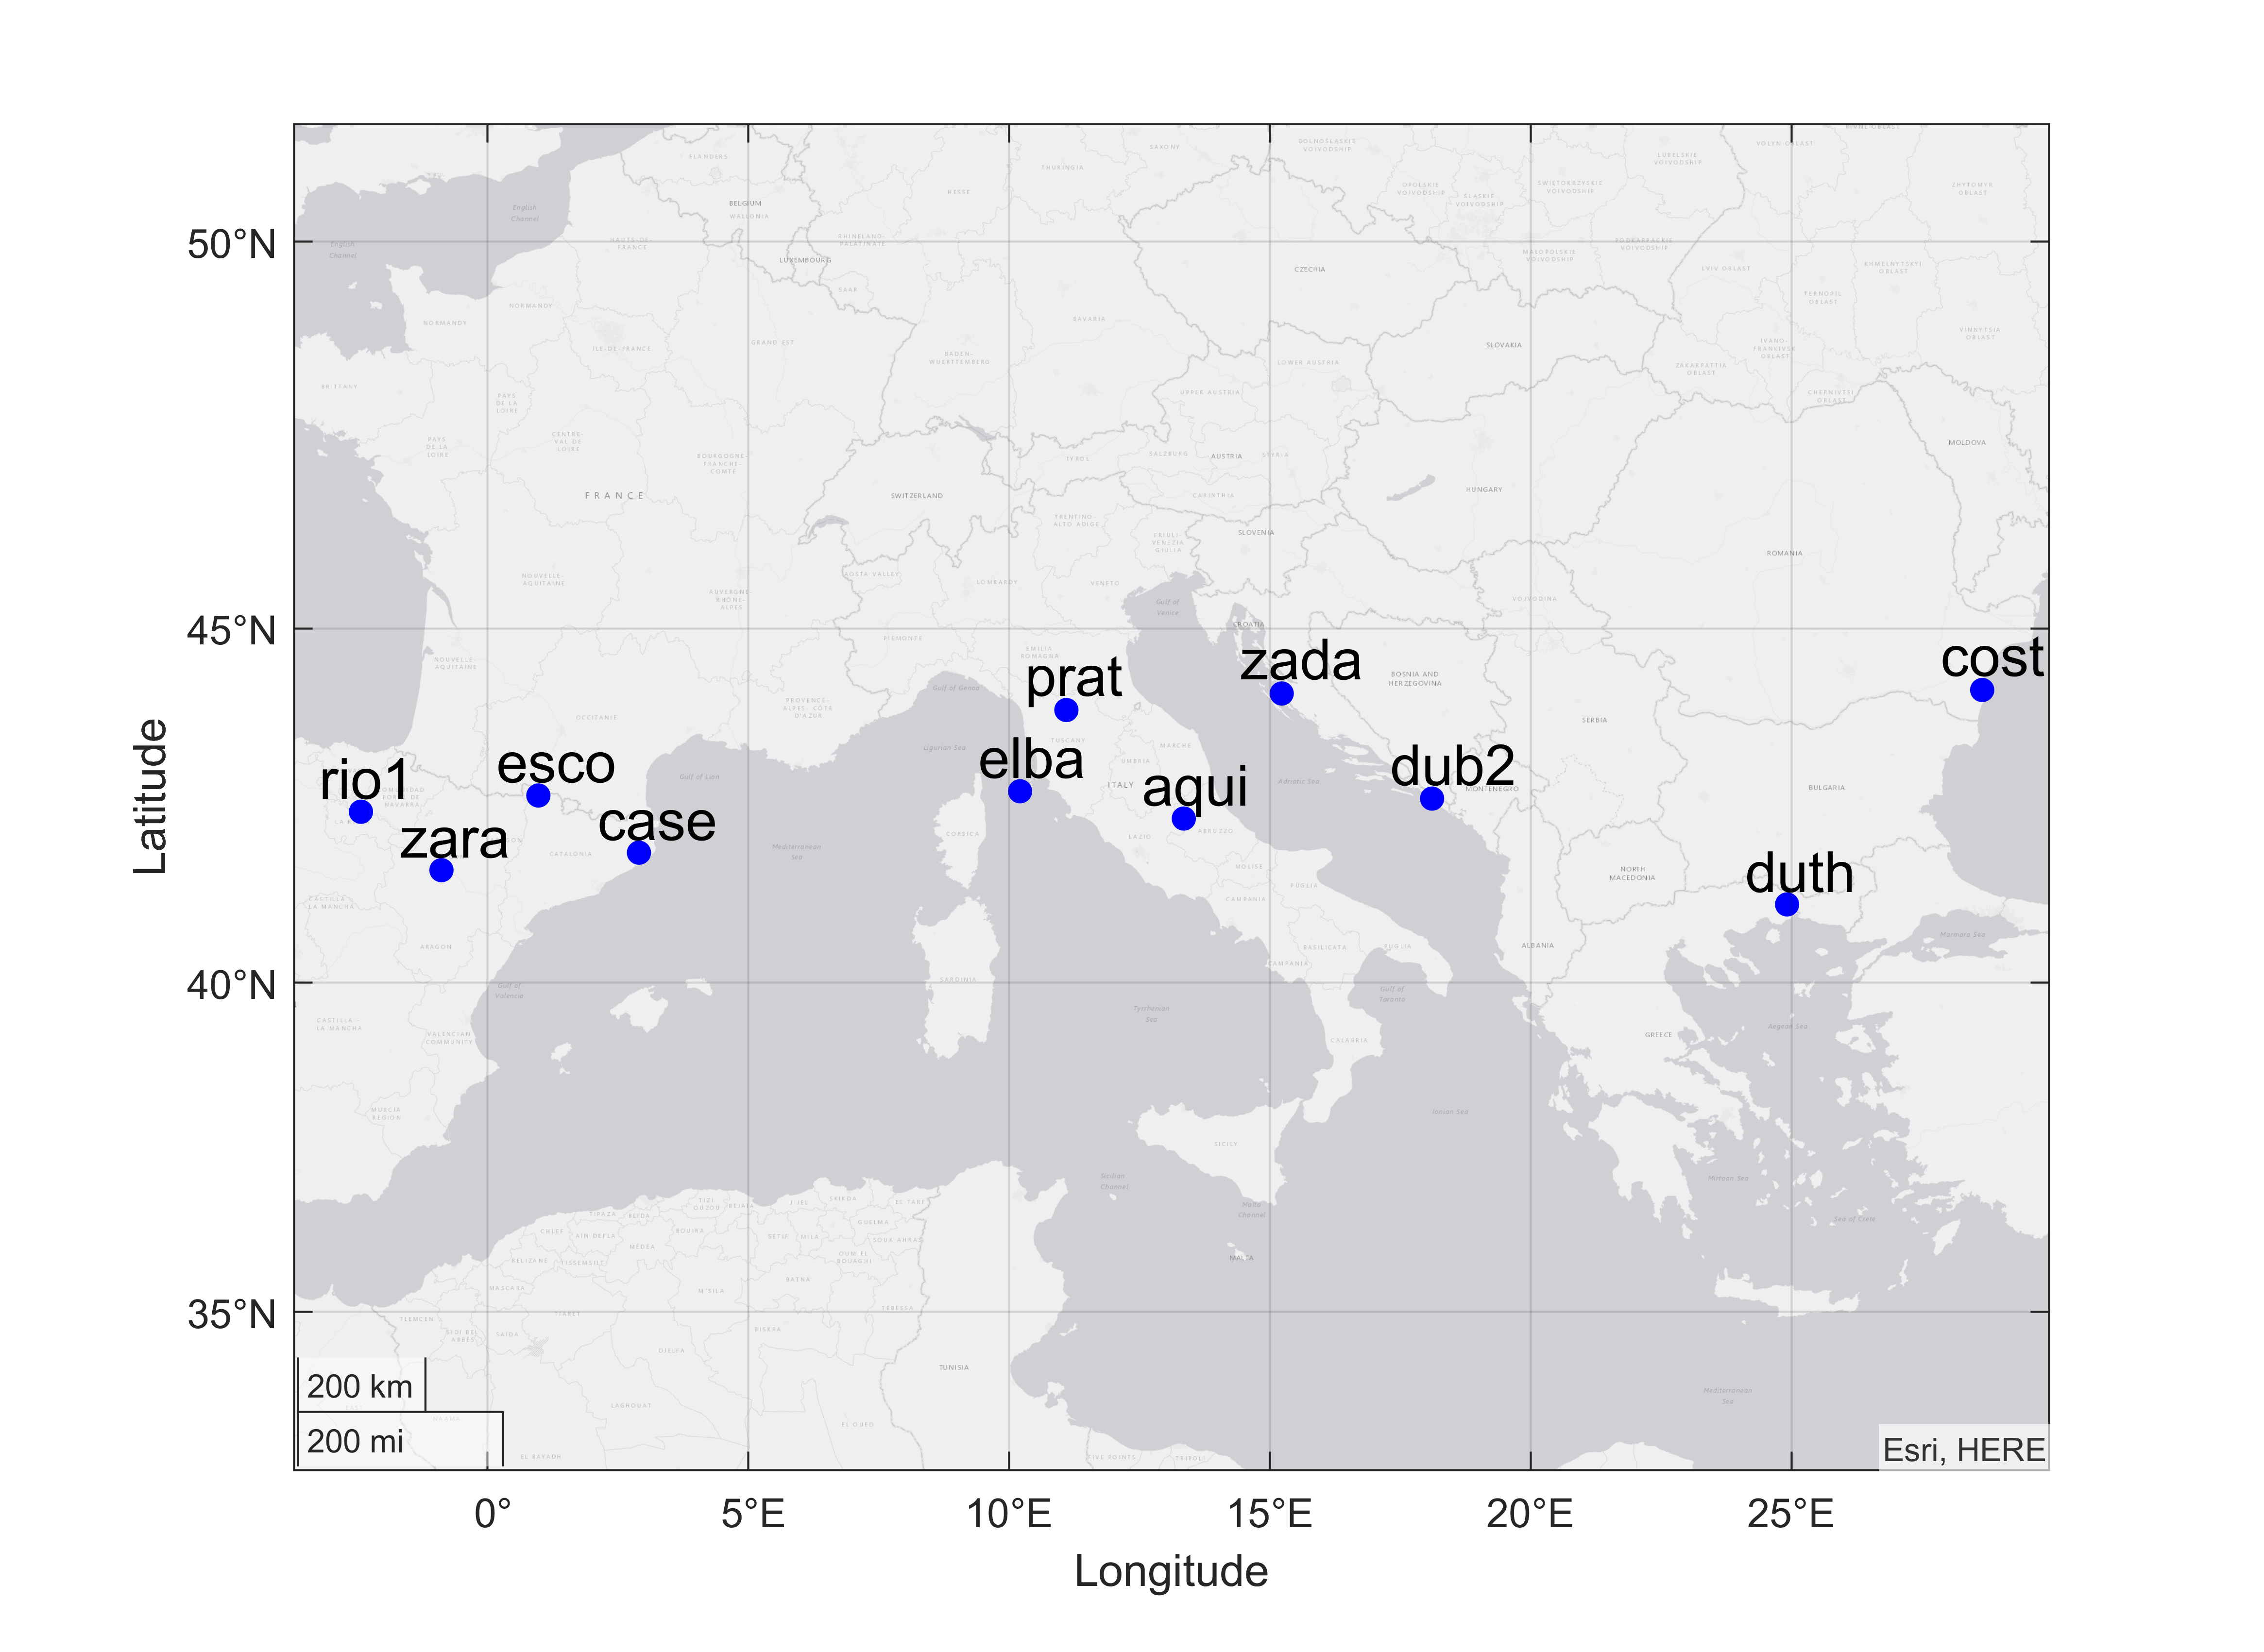
\includegraphics[width = 1\linewidth]{pics/clean_pics/lonStations.png}
\caption{Выбранные станции для долготы}
\label{stationslon}
\end{figure}

\begin{figure}[H]
\centering
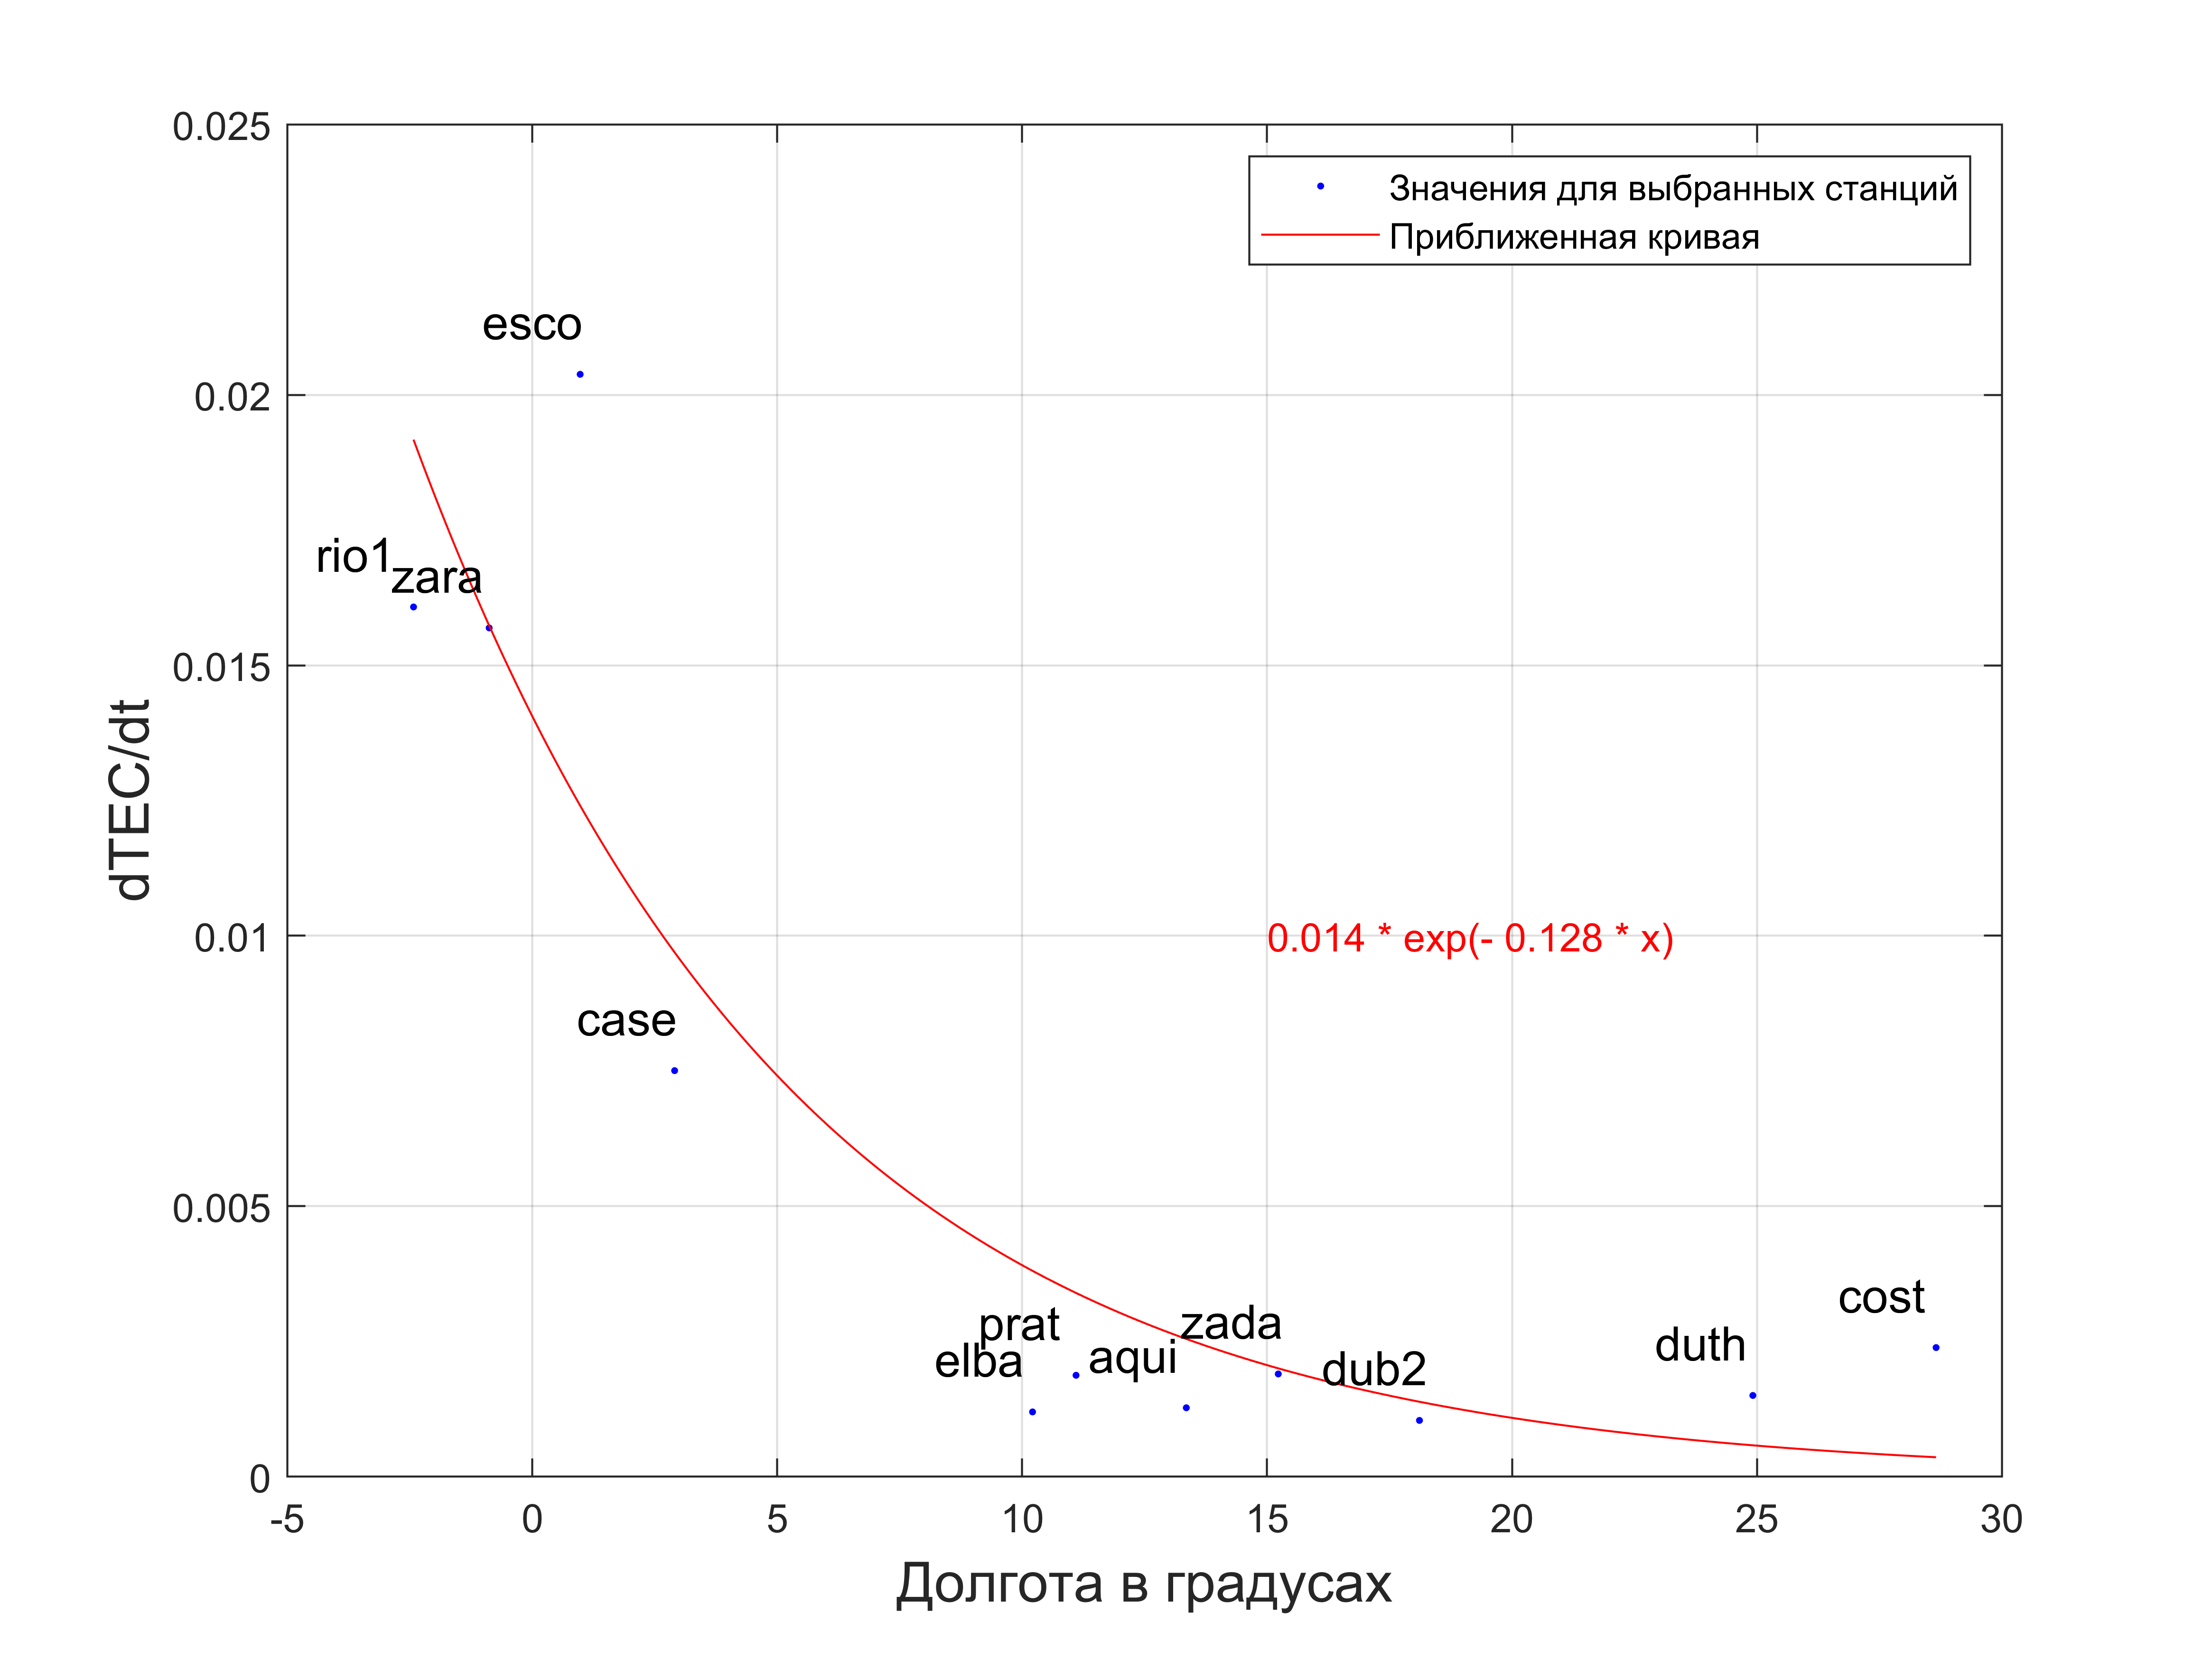
\includegraphics[width = 1\linewidth]{pics/clean_pics/dtec_lon.png}
\caption{Зависимость пикового значения временной производной от изменения координаты долготы.}
\label{dteclon}
\end{figure}

Если рассматривать зависимость от изменения координаты широты, то можно заметить рост значения производной при приближении к экватору. Это связано с тем, что станции, расположенные ближе к экватору, сильнее освещены из-за ориентации Земли.

При рассмотрении зависимости от изменения координаты долготы, виден рост значения производной при проходе от востока к западу, что можно связать с тем, что планета повернута к Солнцу станциями, которые находятся западнее остальных.

Полученные данные свидетельствуют о том, что солнечная вспышка имела влияние на состояние ионосферы. Основное воздействие происходило на территориях, которые были наиболее освещены Солнцем. 


\newpage
\section{Заключение}
В данной работе было рассмотрено влияние солнечной вспышки на значение величины полного электронного содержания. В ходе выполнения работы: был освоен алгоритм расчета абсолютного значения ПЭС, а также пространственно-временных градиентов ПЭС первого и второго порядка по данным приемника ГНСС, расположенного в ГФО "Михнево"; была проведена верификация полученных результатов с данными мировых сетей, которая свидетельствует о том, что данный метод можно считать достоверным; было получено пространственно-временное распределение вариации ПЭС во время солнечной вспышки, свидетельствующее о том, что высокая солнечная активность влияет на состояние ионосферы.


\newpage
\printbibliography

\end{document}
